% Created 2023-06-09 Fri 11:33
\documentclass[9pt, b5paper]{article}
\usepackage{xeCJK}
\usepackage[T1]{fontenc}
\usepackage{bera}
\usepackage[scaled]{beraserif}
\usepackage[scaled]{berasans}
\usepackage[scaled]{beramono}
\usepackage[cache=false]{minted}
\usepackage{xltxtra}
\usepackage{graphicx}
\usepackage{xcolor}
\usepackage{multirow}
\usepackage{multicol}
\usepackage{float}
\usepackage{textcomp}
\usepackage{algorithm}
\usepackage{algorithmic}
\usepackage{latexsym}
\usepackage{natbib}
\usepackage{geometry}
\geometry{left=1.2cm,right=1.2cm,top=1.5cm,bottom=1.2cm}
\usepackage[xetex,colorlinks=true,CJKbookmarks=true,linkcolor=blue,urlcolor=blue,menucolor=blue]{hyperref}
\newminted{common-lisp}{fontsize=\footnotesize} 
\author{deepwaterooo}
\date{\today}
\title{ET 框架学习笔记(三)--网络交互相关}
\hypersetup{
  pdfkeywords={},
  pdfsubject={},
  pdfcreator={Emacs 28.2 (Org mode 8.2.7c)}}
\begin{document}

\maketitle
\tableofcontents


\section{Actor 消息相关}
\label{sec-1}
\subsection{ActorMessageSender: 知道对方的instanceId,使用这个类发actor消息}
\label{sec-1-1}
\begin{itemize}
\item Tcs 成员变量:精华在这里:因为内部自带一个IActorResponse 的异步任务成员变量,可以帮助实现异步消息的自动回复
\item 正是因为内部成员自带一个异步任务,所以会多一个成员变量,就是标记是否要抛异常。这是异步任务成员变量带来的
\begin{minted}[fontsize=\scriptsize,linenos=false]{csharp}
public readonly struct ActorMessageSender {
    public long ActorId { get; }
    public long CreateTime { get; } // 最近接收或者发送消息的时间
    public IActorRequest Request { get; }
    public bool NeedException { get; }
    public ETTask<IActorResponse> Tcs { get; } // <<<<<<<<<<<<<<<<<<<< 精华在这里:因为内部自带一个IActorResponse 的异步任务成员变量,可以帮助实现异步消息的自动回复
    public ActorMessageSender(long actorId, IActorRequest iActorRequest, ETTask<IActorResponse> tcs, bool needException) { // tv ... 
        this.ActorId = actorId;
        this.Request = iActorRequest;
        this.CreateTime = TimeHelper.ServerNow();
        this.Tcs = tcs;
        this.NeedException = needException;
    }
}
\end{minted}
\end{itemize}
\subsection{ActorMessageSenderComponent:}
\label{sec-1-2}
\begin{minted}[fontsize=\scriptsize,linenos=false]{csharp}
[ComponentOf(typeof(Scene))]
public class ActorMessageSenderComponent: Entity, IAwake, IDestroy {
    public const long TIMEOUT_TIME = 40 * 1000;
    public static ActorMessageSenderComponent Instance { get; set; }
    public int RpcId;
    public readonly SortedDictionary<int, ActorMessageSender> requestCallback = new SortedDictionary<int, ActorMessageSender>();
    public long TimeoutCheckTimer;
    public List<int> TimeoutActorMessageSenders = new List<int>();
}
\end{minted}
\subsection{ActorMessageSenderComponentSystem: 这个类ETTask 的细节,要再多看几遍}
\label{sec-1-3}
\begin{itemize}
\item 这个类,可以看见ET7 框架更为系统化、消息机制的更为往底层或说更进一步的封装,就是今天下午看见的,以前的 handle() 或是 run() 方法,或回调实例 Action<T> reply, 现在的封装里,这些什么创建回复实例之类的,全部封装到了管理器或是帮助类
\item 比如这里, check() 方法里,返回消息的实例,已经是自动化系统化地封装了
\item 如果发向同一个进程,则直接处理,不需要通过网络层。内网组件处理内网消息:这个分支可以再跟一下源码,理解一下重构的事件机制流程
\begin{minted}[fontsize=\scriptsize,linenos=false]{csharp}
[FriendOf(typeof(ActorMessageSenderComponent))]
public static class ActorMessageSenderComponentSystem {
    [Invoke(TimerInvokeType.ActorMessageSenderChecker)] // 另一个新标签,激活系
    public class ActorMessageSenderChecker: ATimer<ActorMessageSenderComponent> {
        protected override void Run(ActorMessageSenderComponent self) {
            try {
                self.Check();
            }
            catch (Exception e) {
                Log.Error($"move timer error: {self.Id}\n{e}");
            }
        }
    }
    // [ObjectSystem]// 这里把Awake() Destroy() 方法跳过,不是重点
// 下面的方法是:帮助发送回复消息?好像不对,感觉异步任务结果已经出来了,只差最后写结果的步骤。结果是什么时候执行的?
    private static void Run(ActorMessageSender self, IActorResponse response) { // 传进来的参数:是一个IActorResponse 实例 
        if (response.Error == ErrorCore.ERR_ActorTimeout) {
            self.Tcs.SetException(new Exception($"Rpc error: request, 注意Actor消息超时,请注意查看是否死锁或者没有reply: actorId: {self.ActorId} {self.Request}, response: {response}"));
            return;
        }
        // ActorMessageSenderComponent 一个组件,一次只执行一个(返回)消息发送任务,成员变量永远只管当前任务,也是因为Actor 机制是并行的,一个使者一次只能发一个消息 ...
        if (self.NeedException && ErrorCore.IsRpcNeedThrowException(response.Error)) { // 若是有异常,就先抛异常
            self.Tcs.SetException(new Exception($"Rpc error: actorId: {self.ActorId} request: {self.Request}, response: {response}"));
            return;
        }
        self.Tcs.SetResult(response); // 写结果:把异步任务的状态设置为完成,并触发必要的非空回调订阅者
    }
    private static void Check(this ActorMessageSenderComponent self) {
        long timeNow = TimeHelper.ServerNow();
        foreach ((int key, ActorMessageSender value) in self.requestCallback) {
            // 因为是顺序发送的,所以,检测到第一个不超时的就退出
            if (timeNow < value.CreateTime + ActorMessageSenderComponent.TIMEOUT_TIME) 
                break;
            self.TimeoutActorMessageSenders.Add(key);
        }
        foreach (int rpcId in self.TimeoutActorMessageSenders) {
            ActorMessageSender actorMessageSender = self.requestCallback[rpcId];
            self.requestCallback.Remove(rpcId);
            try {
                IActorResponse response = ActorHelper.CreateResponse(actorMessageSender.Request, ErrorCore.ERR_ActorTimeout);
                Run(actorMessageSender, response);
            }
            catch (Exception e) {
                Log.Error(e.ToString());
            }
        }
        self.TimeoutActorMessageSenders.Clear();
    }
    public static void Send(this ActorMessageSenderComponent self, long actorId, IMessage message) { // 发消息 
        if (actorId == 0) {
            throw new Exception($"actor id is 0: {message}");
        }
        ProcessActorId processActorId = new(actorId);
        // 这里做了优化,如果发向同一个进程,则直接处理,不需要通过网络层
        if (processActorId.Process == Options.Instance.Process) { // 没看懂:这里怎么就说,消息是发向同一进程的了?
            NetInnerComponent.Instance.HandleMessage(actorId, message);
            return;
        }
        Session session = NetInnerComponent.Instance.Get(processActorId.Process);
        session.Send(processActorId.ActorId, message);
    }
    public static int GetRpcId(this ActorMessageSenderComponent self) {
        return ++self.RpcId;
    }
    public static async ETTask<IActorResponse> Call(
        this ActorMessageSenderComponent self,
        long actorId,
        IActorRequest request,
        bool needException = true
        ) {
        request.RpcId = self.GetRpcId();
        if (actorId == 0) {
            throw new Exception($"actor id is 0: {request}");
        }
        return await self.Call(actorId, request.RpcId, request, needException);
    }
    public static async ETTask<IActorResponse> Call( // 发消息:细节比较难懂。感觉还是对ETTask 异步任务没能理解透彻
        this ActorMessageSenderComponent self,
        long actorId,
        int rpcId,
        IActorRequest iActorRequest,
        bool needException = true
        ) {
        if (actorId == 0) {
            throw new Exception($"actor id is 0: {iActorRequest}");
        }
        var tcs = ETTask<IActorResponse>.Create(true); // 对象池里:取一个异步任务。用这个异步作务实例,去创建下面的消息发送者实例
        self.requestCallback.Add(rpcId, new ActorMessageSender(actorId, iActorRequest, tcs, needException)); // 对照发返回消息,再看一遍
        self.Send(actorId, iActorRequest); // 把请求消息发出去
        long beginTime = TimeHelper.ServerFrameTime();
// 【难点】:两个类,当前类,与ETTask,感觉每个词都看懂了,下面一行,连一起,就不明白,它在干什么?
        // 自己想一下的话:异步消息发出去,某个服会处理,有返回消息的话,这个服处理后会返回一个返回消息。
        // 那么下面一行,不是等待创建 Create() 异步任务,是等待这个处理发送消息的服,返回来返回消息,或说把返回消息的内容填好,应该还没发回到消息发送者 
        IActorResponse response = await tcs; // 【稀里糊涂,有点儿不懂】:等异步任务的创建完成,实际是等处理发送消息的服,处理完并写好返回消息
        long endTime = TimeHelper.ServerFrameTime();
        long costTime = endTime - beginTime;
        if (costTime > 200) {
            Log.Warning($"actor rpc time > 200: {costTime} {iActorRequest}");
        }
        return response;
    }
    // 下面方法:处理IActorResponse 消息,也就是,发回复消息给收消息的人XX, 那么谁发,怎么发,就是这个方法的定义
    public static void HandleIActorResponse(this ActorMessageSenderComponent self, IActorResponse response) {
        ActorMessageSender actorMessageSender;
// 下面取、实例化 ActorMessageSender 来看,感觉收消息的 rpcId, 与消息发送者 ActorMessageSender 成一一对应关系。上面的Call() 方法里,创建实例化消息发送者就是这么创始垢 
        if (!self.requestCallback.TryGetValue(response.RpcId, out actorMessageSender)) { // 这里取不到,是说,这个返回消息的发送已经被处理了?
            return;
        }
        self.requestCallback.Remove(response.RpcId); // 这个有序字典,就成为实时更新:随时添加,随时删除
        Run(actorMessageSender, response);
    }
}
\end{minted}
\end{itemize}
\subsection{LocationProxyComponent: 这个代理,什么情况下会用到?}
\label{sec-1-4}
\begin{itemize}
\item 就是有个启动类管理 StartSceneConfigCategory 类,它会分门别类地管理一些什么网关、注册登录服,地址服之类的东西。然后从这个里面拿位置服务器地址?大概意思是这样。
\item 这个类先前仔细读过。还记得小伙伴搬家吗?有的小伙伴搬得狠慢,要花狠久,它搬家过程中就要上锁。大致是这类位置转移管理,位置添加、更新等相关管理操作。
\begin{minted}[fontsize=\scriptsize,linenos=false]{csharp}
[ComponentOf(typeof(Scene))]
public class LocationProxyComponent: Entity, IAwake, IDestroy {
    [StaticField]
    public static LocationProxyComponent Instance;
}
\end{minted}
\end{itemize}
\subsection{LocationProxyComponentSystem}
\label{sec-1-5}
\begin{minted}[fontsize=\scriptsize,linenos=false]{csharp}
// [ObjectSystem] awake() etc
public static class LocationProxyComponentSystem {
    private static long GetLocationSceneId(long key) {
        return StartSceneConfigCategory.Instance.LocationConfig.InstanceId;
    }
    public static async ETTask Add(this LocationProxyComponent self, long key, long instanceId) {
        await ActorMessageSenderComponent.Instance
            .Call(GetLocationSceneId(key),
                  new ObjectAddRequest() { Key = key, InstanceId = instanceId });
    }
    public static async ETTask Lock(this LocationProxyComponent self, long key, long instanceId, int time = 60000) {
        await ActorMessageSenderComponent.Instance
            .Call(GetLocationSceneId(key),
                  new ObjectLockRequest() { Key = key, InstanceId = instanceId, Time = time });
    }
    public static async ETTask UnLock(this LocationProxyComponent self, long key, long oldInstanceId, long instanceId) {
        await ActorMessageSenderComponent.Instance
            .Call(GetLocationSceneId(key),
                  new ObjectUnLockRequest() { Key = key, OldInstanceId = oldInstanceId, InstanceId = instanceId });
    }
    public static async ETTask Remove(this LocationProxyComponent self, long key) {
        await ActorMessageSenderComponent.Instance
            .Call(GetLocationSceneId(key),
                  new ObjectRemoveRequest() { Key = key });
    }
    public static async ETTask<long> Get(this LocationProxyComponent self, long key) {
        if (key == 0) 
            throw new Exception($"get location key 0");
        // location server配置到共享区,一个大战区可以配置N多个location server,这里暂时为1
        ObjectGetResponse response = (ObjectGetResponse) await ActorMessageSenderComponent.Instance
            .Call(GetLocationSceneId(key),
                new ObjectGetRequest() { Key = key });
        return response.InstanceId;
    }
    public static async ETTask AddLocation(this Entity self) {
        await LocationProxyComponent.Instance.Add(self.Id, self.InstanceId);
    }
    public static async ETTask RemoveLocation(this Entity self) {
        await LocationProxyComponent.Instance.Remove(self.Id);
    }
}
\end{minted}
\subsection{ActorLocationSender: 知道对方的Id,使用这个类发actor消息}
\label{sec-1-6}
\begin{minted}[fontsize=\scriptsize,linenos=false]{csharp}
[ChildOf(typeof(ActorLocationSenderComponent))]
public class ActorLocationSender: Entity, IAwake, IDestroy {
    public long ActorId;
    public long LastSendOrRecvTime; // 最近接收或者发送消息的时间
    public int Error;
}
\end{minted}
\subsection{ActorLocationSenderComponent: 位置发送组件}
\label{sec-1-7}
\begin{minted}[fontsize=\scriptsize,linenos=false]{csharp}
 [ComponentOf(typeof(Scene))]
 public class ActorLocationSenderComponent: Entity, IAwake, IDestroy {
     public const long TIMEOUT_TIME = 60 * 1000;
     public static ActorLocationSenderComponent Instance { get; set; }
     public long CheckTimer;
 }
\end{minted}
\subsection{ActorLocationSenderComponentSystem: 这个类,也要明天上午再看一下}
\label{sec-1-8}
\begin{minted}[fontsize=\scriptsize,linenos=false]{csharp}
[Invoke(TimerInvokeType.ActorLocationSenderChecker)]
public class ActorLocationSenderChecker: ATimer<ActorLocationSenderComponent> {
    protected override void Run(ActorLocationSenderComponent self) {
        try {
            self.Check();
        }
        catch (Exception e) {
            Log.Error($"move timer error: {self.Id}\n{e}");
        }
    }
}
// [ObjectSystem] // ...
[FriendOf(typeof(ActorLocationSenderComponent))]
[FriendOf(typeof(ActorLocationSender))]
public static class ActorLocationSenderComponentSystem {
    public static void Check(this ActorLocationSenderComponent self) {
        using (ListComponent<long> list = ListComponent<long>.Create()) {
            long timeNow = TimeHelper.ServerNow();
            foreach ((long key, Entity value) in self.Children) {
                ActorLocationSender actorLocationMessageSender = (ActorLocationSender) value;
                if (timeNow > actorLocationMessageSender.LastSendOrRecvTime + ActorLocationSenderComponent.TIMEOUT_TIME) 
                    list.Add(key);
            }
            foreach (long id in list) {
                self.Remove(id);
            }
        }
    }
    private static ActorLocationSender GetOrCreate(this ActorLocationSenderComponent self, long id) {
        if (id == 0) 
            throw new Exception($"actor id is 0");
        if (self.Children.TryGetValue(id, out Entity actorLocationSender)) {
            return (ActorLocationSender) actorLocationSender;
        }
        actorLocationSender = self.AddChildWithId<ActorLocationSender>(id);
        return (ActorLocationSender) actorLocationSender;
    }
    private static void Remove(this ActorLocationSenderComponent self, long id) {
        if (!self.Children.TryGetValue(id, out Entity actorMessageSender)) 
            return;
        actorMessageSender.Dispose();
    }
    public static void Send(this ActorLocationSenderComponent self, long entityId, IActorRequest message) {
        self.Call(entityId, message).Coroutine();
    }
    public static async ETTask<IActorResponse> Call(this ActorLocationSenderComponent self, long entityId, IActorRequest iActorRequest) {
        ActorLocationSender actorLocationSender = self.GetOrCreate(entityId);
        // 先序列化好
        int rpcId = ActorMessageSenderComponent.Instance.GetRpcId();
        iActorRequest.RpcId = rpcId;
        long actorLocationSenderInstanceId = actorLocationSender.InstanceId;
        using (await CoroutineLockComponent.Instance.Wait(CoroutineLockType.ActorLocationSender, entityId)) {
            if (actorLocationSender.InstanceId != actorLocationSenderInstanceId) 
                throw new RpcException(ErrorCore.ERR_ActorTimeout, $"{iActorRequest}");
            // 队列中没处理的消息返回跟上个消息一样的报错
            if (actorLocationSender.Error == ErrorCore.ERR_NotFoundActor) 
                return ActorHelper.CreateResponse(iActorRequest, actorLocationSender.Error);
            try {
                return await self.CallInner(actorLocationSender, rpcId, iActorRequest);
            }
            catch (RpcException) {
                self.Remove(actorLocationSender.Id);
                throw;
            }
            catch (Exception e) {
                self.Remove(actorLocationSender.Id);
                throw new Exception($"{iActorRequest}", e);
            }
        }
    }
    private static async ETTask<IActorResponse> CallInner(this ActorLocationSenderComponent self, ActorLocationSender actorLocationSender, int rpcId, IActorRequest iActorRequest) {
        int failTimes = 0;
        long instanceId = actorLocationSender.InstanceId;
        actorLocationSender.LastSendOrRecvTime = TimeHelper.ServerNow();
        while (true) {
            if (actorLocationSender.ActorId == 0) {
                actorLocationSender.ActorId = await LocationProxyComponent.Instance.Get(actorLocationSender.Id);
                if (actorLocationSender.InstanceId != instanceId) 
                    throw new RpcException(ErrorCore.ERR_ActorLocationSenderTimeout2, $"{iActorRequest}");
            }
            if (actorLocationSender.ActorId == 0) {
                actorLocationSender.Error = ErrorCore.ERR_NotFoundActor;
                return ActorHelper.CreateResponse(iActorRequest, ErrorCore.ERR_NotFoundActor);
            }
            IActorResponse response = await ActorMessageSenderComponent.Instance.Call(actorLocationSender.ActorId, rpcId, iActorRequest, false);
            if (actorLocationSender.InstanceId != instanceId) 
                throw new RpcException(ErrorCore.ERR_ActorLocationSenderTimeout3, $"{iActorRequest}");
            switch (response.Error) {
                case ErrorCore.ERR_NotFoundActor: {
                    // 如果没找到Actor,重试
                    ++failTimes;
                    if (failTimes > 20) {
                        Log.Debug($"actor send message fail, actorid: {actorLocationSender.Id}");
                        actorLocationSender.Error = ErrorCore.ERR_NotFoundActor;
                        // 这里不能删除actor,要让后面等待发送的消息也返回ERR_NotFoundActor,直到超时删除
                        return response;
                    }
                    // 等待0.5s再发送
                    await TimerComponent.Instance.WaitAsync(500);
                    if (actorLocationSender.InstanceId != instanceId)
                        throw new RpcException(ErrorCore.ERR_ActorLocationSenderTimeout4, $"{iActorRequest}");
                    actorLocationSender.ActorId = 0;
                    continue;
                }
                case ErrorCore.ERR_ActorTimeout: 
                    throw new RpcException(response.Error, $"{iActorRequest}");
            }
            if (ErrorCore.IsRpcNeedThrowException(response.Error)) {
                throw new RpcException(response.Error, $"Message: {response.Message} Request: {iActorRequest}");
            }
            return response;
        }
    }
}
\end{minted}
\subsection{ActorHelper: 帮助创建IActorResponse 回复消息。狠简单}
\label{sec-1-9}
\begin{minted}[fontsize=\scriptsize,linenos=false]{csharp}
public static class ActorHelper {
    public static IActorResponse CreateResponse(IActorRequest iActorRequest, int error) {
        Type responseType = OpcodeTypeComponent.Instance.GetResponseType(iActorRequest.GetType());
        IActorResponse response = (IActorResponse)Activator.CreateInstance(responseType);
        response.Error = error;
        response.RpcId = iActorRequest.RpcId;
        return response;
    }
}
\end{minted}
\subsection{ActorMessageDispatcherInfo | ActorMessageDispatcherComponent}
\label{sec-1-10}
\begin{minted}[fontsize=\scriptsize,linenos=false]{csharp}
public class ActorMessageDispatcherInfo {
    public SceneType SceneType { get; }
    public IMActorHandler IMActorHandler { get; }
    public ActorMessageDispatcherInfo(SceneType sceneType, IMActorHandler imActorHandler) {
        this.SceneType = sceneType;
        this.IMActorHandler = imActorHandler;
    }
}
[ComponentOf(typeof(Scene))] // Actor消息分发组件
public class ActorMessageDispatcherComponent: Entity, IAwake, IDestroy, ILoad {
    [StaticField]
    public static ActorMessageDispatcherComponent Instance;
    public readonly Dictionary<Type, List<ActorMessageDispatcherInfo>> ActorMessageHandlers = new();
}
\end{minted}
\subsection{ActorMessageDispatcherComponentHelper: 帮助类}
\label{sec-1-11}
\begin{itemize}
\item Actor消息分发组件:对于管理器里的,对同一发送消息类型,不同场景下不同处理器的链表管理,多看几遍
\item 这里,对于同一发送消息类型, 是会、是可能存在【从不同的场景类型中返回,带不同的消息处理器】 以致于必须得链表管理同一发送消息类型的不同可能处理情况。
\begin{minted}[fontsize=\scriptsize,linenos=false]{csharp}
[FriendOf(typeof(ActorMessageDispatcherComponent))] // Actor消息分发组件:对于管理器里的,对同一发送消息类型,不同场景下不同处理器的链表管理,多看几遍
public static class ActorMessageDispatcherComponentHelper {// Awake() Load() Destroy() 省略掉了
    private static void Load(this ActorMessageDispatcherComponent self) { // 加载:程序域回载的时候
        self.ActorMessageHandlers.Clear(); // 清空字典 
        var types = EventSystem.Instance.GetTypes(typeof (ActorMessageHandlerAttribute)); // 扫描程序域里的特定消息处理器标签 
        foreach (Type type in types) {
            object obj = Activator.CreateInstance(type); // 加载时:框架封装,自动创建【消息处理器】实例
            IMActorHandler imHandler = obj as IMActorHandler;
            if (imHandler == null) {
                throw new Exception($"message handler not inherit IMActorHandler abstract class: {obj.GetType().FullName}");
            }
            object[] attrs = type.GetCustomAttributes(typeof(ActorMessageHandlerAttribute), false);
            foreach (object attr in attrs) {
                ActorMessageHandlerAttribute actorMessageHandlerAttribute = attr as ActorMessageHandlerAttribute;
                Type messageType = imHandler.GetRequestType(); // 因为消息处理接口的封装:可以拿到发送类型
                Type handleResponseType = imHandler.GetResponseType();// 因为消息处理接口的封装:可以拿到返回消息的类型
                if (handleResponseType != null) {
                    Type responseType = OpcodeTypeComponent.Instance.GetResponseType(messageType);
                    if (handleResponseType != responseType) {
                        throw new Exception($"message handler response type error: {messageType.FullName}");
                    }
                }
                // 将必要的消息【发送类型】【返回类型】存起来,统一管理,备用
                // 这里,对于同一发送消息类型, 是会、是可能存在【从不同的场景类型中返回,带不同的消息处理器】 以致于必须得链表管理
                // 这里,感觉因为想不到、从概念上也地无法理解,可能会存在的适应情况、上下文场景,所以这里的链表管理同一发送消息类型,理解起来还有点儿困难
                ActorMessageDispatcherInfo actorMessageDispatcherInfo = new(actorMessageHandlerAttribute.SceneType, imHandler);
                self.RegisterHandler(messageType, actorMessageDispatcherInfo); // 存在本管理组件,所管理的字典里
            }
        }
    }
    private static void RegisterHandler(this ActorMessageDispatcherComponent self, Type type, ActorMessageDispatcherInfo handler) {
        // 这里,对于同一发送消息类型, 是会、是可能存在【从不同的场景类型中返回,带不同的消息处理器】 以致于必须得链表管理
        // 这里,感觉因为想不到、从概念上也地无法理解,可能会存在的适应情况、上下文场景,所以这里的链表管理同一发送消息类型,理解起来还有点儿困难
        if (!self.ActorMessageHandlers.ContainsKey(type)) 
            self.ActorMessageHandlers.Add(type, new List<ActorMessageDispatcherInfo>());
        self.ActorMessageHandlers[type].Add(handler);
    }
    public static async ETTask Handle(this ActorMessageDispatcherComponent self, Entity entity, int fromProcess, object message) {
        List<ActorMessageDispatcherInfo> list;
        if (!self.ActorMessageHandlers.TryGetValue(message.GetType(), out list)) // 根据消息的发送类型,来取所有可能的处理器包装链表 
            throw new Exception($"not found message handler: {message}");
        SceneType sceneType = entity.DomainScene().SceneType; // 定位:当前消息的场景类型
        foreach (ActorMessageDispatcherInfo actorMessageDispatcherInfo in list) { // 遍历:这个发送消息类型,所有存在注册过的消息处理器封装
            if (actorMessageDispatcherInfo.SceneType != sceneType)  // 场景不符就跳过
                continue;
            // 定位:是当前特定场景下的消息处理器,那么,就调用这个处理器,要它去干事。【爱表哥,爱生活!!!任何时候,活宝妹就是一定要嫁给亲爱的表哥!!!】
            await actorMessageDispatcherInfo.IMActorHandler.Handle(entity, fromProcess, message);   
        }
    }
}
\end{minted}
\end{itemize}
\subsection{ActorMessageHandlerAttribute 标签系: 去找几个典型标签看看}
\label{sec-1-12}
\begin{minted}[fontsize=\scriptsize,linenos=false]{csharp}
public class ActorMessageHandlerAttribute: BaseAttribute {
    public SceneType SceneType { get; }
    public ActorMessageHandlerAttribute(SceneType sceneType) {
        this.SceneType = sceneType;
    }
}
\end{minted}
\subsection{[ActorMessageHandler(SceneType.Gate)] 标签使用举例}
\label{sec-1-13}
\begin{itemize}
\item 是以前框架中或是参考项目中的例子。标签使用申明说,这是【网关服】上的一个Actor 消息处理器定义类。
\begin{minted}[fontsize=\scriptsize,linenos=false]{csharp}
[ActorMessageHandler(SceneType.Gate)]
public class Actor_MatchSucess_NttHandler : AMActorHandler<User, Actor_MatchSucess_Ntt> {
    protected override void Run(User user, Actor_MatchSucess_Ntt message) {
        user.IsMatching = false;
        user.ActorID = message.GamerID;
        Log.Info($"玩家{user.UserID}匹配成功");
    }
}
\end{minted}
\end{itemize}
\subsection{MailBoxComponent: 挂上这个组件表示该Entity是一个Actor,接收的消息将会队列处理}
\label{sec-1-14}
\begin{minted}[fontsize=\scriptsize,linenos=false]{csharp}
// 挂上这个组件表示该Entity是一个Actor,接收的消息将会队列处理
[ComponentOf]
public class MailBoxComponent: Entity, IAwake, IAwake<MailboxType> {
    // Mailbox的类型
    public MailboxType MailboxType { get; set; }
}
\end{minted}
\subsection{MailboxType}
\label{sec-1-15}
\begin{minted}[fontsize=\scriptsize,linenos=false]{csharp}
public enum MailboxType {
    MessageDispatcher, // 消息分发器
    UnOrderMessageDispatcher,// 无序分发
    GateSession,// 网关?
}
\end{minted}
\subsection{【服务端】ActorHandleHelper 帮助类。【需要去深挖一下】}
\label{sec-1-16}
\begin{minted}[fontsize=\scriptsize,linenos=false]{csharp}
public static class ActorHandleHelper {
    public static void Reply(int fromProcess, IActorResponse response) {
        if (fromProcess == Options.Instance.Process) { // 返回消息是同一个进程
            // NetInnerComponent.Instance.HandleMessage(realActorId, response); // 等同于直接调用下面这句【我自己暂时放回来的】
            ActorMessageSenderComponent.Instance.HandleIActorResponse(response);
            return;
        }
        Session replySession = NetInnerComponent.Instance.Get(fromProcess);
        replySession.Send(response);
    }
    public static void HandleIActorResponse(IActorResponse response) {
        ActorMessageSenderComponent.Instance.HandleIActorResponse(response);
    }
    // 分发actor消息
    [EnableAccessEntiyChild]
    public static async ETTask HandleIActorRequest(long actorId, IActorRequest iActorRequest) {
        InstanceIdStruct instanceIdStruct = new(actorId);
        int fromProcess = instanceIdStruct.Process;
        instanceIdStruct.Process = Options.Instance.Process;
        long realActorId = instanceIdStruct.ToLong();
        Entity entity = Root.Instance.Get(realActorId);
        if (entity == null) {
            IActorResponse response = ActorHelper.CreateResponse(iActorRequest, ErrorCore.ERR_NotFoundActor);
            Reply(fromProcess, response);
            return;
        }
        MailBoxComponent mailBoxComponent = entity.GetComponent<MailBoxComponent>();
        if (mailBoxComponent == null) {
            Log.Warning($"actor not found mailbox: {entity.GetType().Name} {realActorId} {iActorRequest}");
            IActorResponse response = ActorHelper.CreateResponse(iActorRequest, ErrorCore.ERR_NotFoundActor);
            Reply(fromProcess, response);
            return;
        }
        switch (mailBoxComponent.MailboxType) {
            case MailboxType.MessageDispatcher: {
                using (await CoroutineLockComponent.Instance.Wait(CoroutineLockType.Mailbox, realActorId)) {
                    if (entity.InstanceId != realActorId) {
                        IActorResponse response = ActorHelper.CreateResponse(iActorRequest, ErrorCore.ERR_NotFoundActor);
                        Reply(fromProcess, response);
                        break;
                    }
                    await ActorMessageDispatcherComponent.Instance.Handle(entity, fromProcess, iActorRequest);
                }
                break;
            }
            case MailboxType.UnOrderMessageDispatcher: {
                await ActorMessageDispatcherComponent.Instance.Handle(entity, fromProcess, iActorRequest);
                break;
            }
            case MailboxType.GateSession:
            default:
                throw new Exception($"no mailboxtype: {mailBoxComponent.MailboxType} {iActorRequest}");
        }
    }
    // 分发actor消息
    [EnableAccessEntiyChild]
    public static async ETTask HandleIActorMessage(long actorId, IActorMessage iActorMessage) {
        InstanceIdStruct instanceIdStruct = new(actorId);
        int fromProcess = instanceIdStruct.Process;
        instanceIdStruct.Process = Options.Instance.Process;
        long realActorId = instanceIdStruct.ToLong();
        Entity entity = Root.Instance.Get(realActorId);
        if (entity == null) {
            Log.Error($"not found actor: {realActorId} {iActorMessage}");
            return;
        }
        MailBoxComponent mailBoxComponent = entity.GetComponent<MailBoxComponent>();
        if (mailBoxComponent == null) {
            Log.Error($"actor not found mailbox: {entity.GetType().Name} {realActorId} {iActorMessage}");
            return;
        }
        switch (mailBoxComponent.MailboxType) {
        case MailboxType.MessageDispatcher: {
            using (await CoroutineLockComponent.Instance.Wait(CoroutineLockType.Mailbox, realActorId)) {
                if (entity.InstanceId != realActorId) {
                    break;
                }
                await ActorMessageDispatcherComponent.Instance.Handle(entity, fromProcess, iActorMessage);
            }
            break;
        }
        case MailboxType.UnOrderMessageDispatcher: {
            await ActorMessageDispatcherComponent.Instance.Handle(entity, fromProcess, iActorMessage);
            break;
        }
        case MailboxType.GateSession: {
            if (entity is Session gateSession) {
                // 发送给客户端
                gateSession.Send(iActorMessage);
            }
            break;
        }
        default:
            throw new Exception($"no mailboxtype: {mailBoxComponent.MailboxType} {iActorMessage}");
        }
    }
}
\end{minted}


\section{StartConfigComponent: 找【各种服】的起始初始化地址}
\label{sec-2}
\subsection{ConfigSingleton<T>: ProtoObject, ISingleton}
\label{sec-2-1}
\begin{minted}[fontsize=\scriptsize,linenos=false]{java}
public abstract class ConfigSingleton<T>: ProtoObject, ISingleton where T: ConfigSingleton<T>, new() {
        [StaticField]
        private static T instance;
        public static T Instance {
            get {
                return instance ??= ConfigComponent.Instance.LoadOneConfig(typeof (T)) as T;
            }
        }
        void ISingleton.Register() {
            if (instance != null) {
                throw new Exception($"singleton register twice! {typeof (T).Name}");
            }
            instance = (T)this;
        }
        void ISingleton.Destroy() {
            T t = instance;
            instance = null;
            t.Dispose();
        }
        bool ISingleton.IsDisposed() {
            throw new NotImplementedException();
        }
        public override void AfterEndInit() { }
        public virtual void Dispose() { }
    }
\end{minted}
\subsection{SceneFactory 里可以给【匹配服】添加组件}
\label{sec-2-2}
\begin{minted}[fontsize=\scriptsize,linenos=false]{java}
public static class SceneFactory {
    public static async ETTask<Scene> CreateServerScene(Entity parent, long id, long instanceId, int zone, string name, SceneType sceneType, StartSceneConfig startSceneConfig = null) {
        await ETTask.CompletedTask;
        Scene scene = EntitySceneFactory.CreateScene(id, instanceId, zone, sceneType, name, parent);
        scene.AddComponent<MailBoxComponent, MailboxType>(MailboxType.UnOrderMessageDispatcher);
        switch (scene.SceneType) {
        case SceneType.Router:
            scene.AddComponent<RouterComponent, IPEndPoint, string>(startSceneConfig.OuterIPPort, startSceneConfig.StartProcessConfig.InnerIP);
            break;
        case SceneType.RouterManager: // 正式发布请用CDN代替RouterManager
            // 云服务器在防火墙那里做端口映射
            scene.AddComponent<HttpComponent, string>($"http:// *:{startSceneConfig.OuterPort}/");
            break;
        case SceneType.Realm:
            scene.AddComponent<NetServerComponent, IPEndPoint>(startSceneConfig.InnerIPOutPort);
            break;
        case SceneType.Match: // <<<<<<<<<<<<<<<<<<<< 这里是,我可以添加【匹配服】相关功能组件的地方。【参考项目原原码】感觉被我弄丢了
            break;
        case SceneType.Gate:
            scene.AddComponent<NetServerComponent, IPEndPoint>(startSceneConfig.InnerIPOutPort);
            scene.AddComponent<PlayerComponent>();
            scene.AddComponent<GateSessionKeyComponent>();
            break;
        case SceneType.Map:
            scene.AddComponent<UnitComponent>();
            scene.AddComponent<AOIManagerComponent>();
            break;
        case SceneType.Location:
            scene.AddComponent<LocationComponent>();
            break;
//...
        }
        return scene;
    }
}
\end{minted}
\subsection{RouterAddressComponent: 路由器组件}
\label{sec-2-3}
\begin{minted}[fontsize=\scriptsize,linenos=false]{java}
[ComponentOf(typeof(Scene))]
public class RouterAddressComponent: Entity, IAwake<string, int> {
    public IPAddress RouterManagerIPAddress { get; set; }
    public string RouterManagerHost;
    public int RouterManagerPort;
    public HttpGetRouterResponse Info;
    public int RouterIndex;
}
\end{minted}
\subsection{RouterAddressComponentSystem: 路由器的生成系}
\label{sec-2-4}
\begin{minted}[fontsize=\scriptsize,linenos=false]{java}
[FriendOf(typeof(RouterAddressComponent))]
public static class RouterAddressComponentSystem {
    public class RouterAddressComponentAwakeSystem: AwakeSystem<RouterAddressComponent, string, int> {
        protected override void Awake(RouterAddressComponent self, string address, int port) {
            self.RouterManagerHost = address;
            self.RouterManagerPort = port;
        }
    }
    public static async ETTask Init(this RouterAddressComponent self) {
        self.RouterManagerIPAddress = NetworkHelper.GetHostAddress(self.RouterManagerHost);
        await self.GetAllRouter();
    }
    private static async ETTask GetAllRouter(this RouterAddressComponent self) {
        string url = $"http:// {self.RouterManagerHost}:{self.RouterManagerPort}/get_router?v={RandomGenerator.RandUInt32()}";
        Log.Debug($"start get router info: {url}");
        string routerInfo = await HttpClientHelper.Get(url);
        Log.Debug($"recv router info: {routerInfo}");
        HttpGetRouterResponse httpGetRouterResponse = JsonHelper.FromJson<HttpGetRouterResponse>(routerInfo);
        self.Info = httpGetRouterResponse;
        Log.Debug($"start get router info finish: {JsonHelper.ToJson(httpGetRouterResponse)}");
        // 打乱顺序
        RandomGenerator.BreakRank(self.Info.Routers);
        self.WaitTenMinGetAllRouter().Coroutine();
    }
    // 等10分钟再获取一次
    public static async ETTask WaitTenMinGetAllRouter(this RouterAddressComponent self) {
        await TimerComponent.Instance.WaitAsync(5 * 60 * 1000);
        if (self.IsDisposed) 
            return;
        await self.GetAllRouter();
    }
    public static IPEndPoint GetAddress(this RouterAddressComponent self) {
        if (self.Info.Routers.Count == 0) 
            return null;
        string address = self.Info.Routers[self.RouterIndex++ % self.Info.Routers.Count];
        string[] ss = address.Split(':');
        IPAddress ipAddress = IPAddress.Parse(ss[0]);
        if (self.RouterManagerIPAddress.AddressFamily == AddressFamily.InterNetworkV6) { 
            ipAddress = ipAddress.MapToIPv6();
        }
        return new IPEndPoint(ipAddress, int.Parse(ss[1]));
    }
    public static IPEndPoint GetRealmAddress(this RouterAddressComponent self, string account) { // <<<<<<<<<<<<<<<<<<<< 照葫芦画飘,扩展方法 
        int v = account.Mode(self.Info.Realms.Count);
        string address = self.Info.Realms[v];
        string[] ss = address.Split(':');
        IPAddress ipAddress = IPAddress.Parse(ss[0]);
        // if (self.IPAddress.AddressFamily == AddressFamily.InterNetworkV6) 
        //    ipAddress = ipAddress.MapToIPv6();
        return new IPEndPoint(ipAddress, int.Parse(ss[1]));
    }
}
\end{minted}

\subsection{RouterHelper: 路由器帮助类,向路由器注册、申请?}
\label{sec-2-5}
\begin{minted}[fontsize=\scriptsize,linenos=false]{java}
public static class RouterHelper {
    // 注册router
    public static async ETTask<Session> CreateRouterSession(Scene clientScene, IPEndPoint address) {
        (uint recvLocalConn, IPEndPoint routerAddress) = await GetRouterAddress(clientScene, address, 0, 0);
        if (recvLocalConn == 0) 
            throw new Exception($"get router fail: {clientScene.Id} {address}");
        Log.Info($"get router: {recvLocalConn} {routerAddress}");
        Session routerSession = clientScene.GetComponent<NetClientComponent>().Create(routerAddress, address, recvLocalConn);
        routerSession.AddComponent<PingComponent>();
        routerSession.AddComponent<RouterCheckComponent>();
        return routerSession;
    }
    public static async ETTask<(uint, IPEndPoint)> GetRouterAddress(Scene clientScene, IPEndPoint address, uint localConn, uint remoteConn) {
        Log.Info($"start get router address: {clientScene.Id} {address} {localConn} {remoteConn}");
        // return (RandomHelper.RandUInt32(), address);
        RouterAddressComponent routerAddressComponent = clientScene.GetComponent<RouterAddressComponent>();
        IPEndPoint routerInfo = routerAddressComponent.GetAddress();
        uint recvLocalConn = await Connect(routerInfo, address, localConn, remoteConn);
        Log.Info($"finish get router address: {clientScene.Id} {address} {localConn} {remoteConn} {recvLocalConn} {routerInfo}");
        return (recvLocalConn, routerInfo);
    }
    // 向router申请
    private static async ETTask<uint> Connect(IPEndPoint routerAddress, IPEndPoint realAddress, uint localConn, uint remoteConn) {
        uint connectId = RandomGenerator.RandUInt32();
        using Socket socket = new Socket(routerAddress.AddressFamily, SocketType.Dgram, ProtocolType.Udp);
        int count = 20;
        byte[] sendCache = new byte[512];
        byte[] recvCache = new byte[512];
        uint synFlag = localConn == 0? KcpProtocalType.RouterSYN : KcpProtocalType.RouterReconnectSYN;
        sendCache.WriteTo(0, synFlag);
        sendCache.WriteTo(1, localConn);
        sendCache.WriteTo(5, remoteConn);
        sendCache.WriteTo(9, connectId);
        byte[] addressBytes = realAddress.ToString().ToByteArray();
        Array.Copy(addressBytes, 0, sendCache, 13, addressBytes.Length);
        Log.Info($"router connect: {connectId} {localConn} {remoteConn} {routerAddress} {realAddress}");

        EndPoint recvIPEndPoint = new IPEndPoint(IPAddress.Any, 0);
        long lastSendTimer = 0;
        while (true) {
            long timeNow = TimeHelper.ClientFrameTime();
            if (timeNow - lastSendTimer > 300) {
                if (--count < 0) {
                    Log.Error($"router connect timeout fail! {localConn} {remoteConn} {routerAddress} {realAddress}");
                    return 0;
                }
                lastSendTimer = timeNow;
                // 发送
                socket.SendTo(sendCache, 0, addressBytes.Length + 13, SocketFlags.None, routerAddress);
            }
            await TimerComponent.Instance.WaitFrameAsync();
            // 接收
            if (socket.Available > 0) {
                int messageLength = socket.ReceiveFrom(recvCache, ref recvIPEndPoint);
                if (messageLength != 9) {
                    Log.Error($"router connect error1: {connectId} {messageLength} {localConn} {remoteConn} {routerAddress} {realAddress}");
                    continue;
                }
                byte flag = recvCache[0];
                if (flag != KcpProtocalType.RouterReconnectACK && flag != KcpProtocalType.RouterACK) {
                    Log.Error($"router connect error2: {connectId} {synFlag} {flag} {localConn} {remoteConn} {routerAddress} {realAddress}");
                    continue;
                }
                uint recvRemoteConn = BitConverter.ToUInt32(recvCache, 1);
                uint recvLocalConn = BitConverter.ToUInt32(recvCache, 5);
                Log.Info($"router connect finish: {connectId} {recvRemoteConn} {recvLocalConn} {localConn} {remoteConn} {routerAddress} {realAddress}");
                return recvLocalConn;
            }
        }
    }
}
\end{minted}

\subsection{StartProcessConfigCategory : ConfigSingleton<StartProcessConfigCategory>, IMerge: 【任何时候,活宝妹就是一定要嫁给亲爱的表哥!!!】}
\label{sec-2-6}
\begin{minted}[fontsize=\scriptsize,linenos=false]{java}
[ProtoContract]
[Config]
public partial class StartProcessConfigCategory : ConfigSingleton<StartProcessConfigCategory>, IMerge {
    [ProtoIgnore]
    [BsonIgnore]
    private Dictionary<int, StartProcessConfig> dict = new Dictionary<int, StartProcessConfig>(); // 管理字典
    [BsonElement]
    [ProtoMember(1)]
    private List<StartProcessConfig> list = new List<StartProcessConfig>();
    public void Merge(object o) {
        StartProcessConfigCategory s = o as StartProcessConfigCategory;
        this.list.AddRange(s.list);
    }
    [ProtoAfterDeserialization]        
    public void ProtoEndInit() {
        foreach (StartProcessConfig config in list) {
            config.AfterEndInit();
            this.dict.Add(config.Id, config);
        }
        this.list.Clear();
        this.AfterEndInit();
    }
    public StartProcessConfig Get(int id) {
        this.dict.TryGetValue(id, out StartProcessConfig item);
        if (item == null) {
            throw new Exception($"配置找不到,配置表名: {nameof (StartProcessConfig)},配置id: {id}");
        }
        return item;
    }
    public bool Contain(int id) {
        return this.dict.ContainsKey(id);
    }
    public Dictionary<int, StartProcessConfig> GetAll() {
        return this.dict;
    }
    public StartProcessConfig GetOne() {
        if (this.dict == null || this.dict.Count <= 0) {
            return null;
        }
        return this.dict.Values.GetEnumerator().Current;
    }
}
[ProtoContract]
public partial class StartProcessConfig: ProtoObject, IConfig {
    [ProtoMember(1)]
    public int Id { get; set; }
    [ProtoMember(2)]
    public int MachineId { get; set; }
    [ProtoMember(3)]
    public int InnerPort { get; set; }
}
\end{minted}
\subsection{StartSceneConfig: ISupportInitialize 【各种服-配置,场景配置】}
\label{sec-2-7}
\begin{minted}[fontsize=\scriptsize,linenos=false]{csharp}
public partial class StartSceneConfig: ISupportInitialize {
    public long InstanceId;
    public SceneType Type; // 场景类型

    public StartProcessConfig StartProcessConfig {
        get {
            return StartProcessConfigCategory.Instance.Get(this.Process);
        }
    }
    public StartZoneConfig StartZoneConfig {
        get {
            return StartZoneConfigCategory.Instance.Get(this.Zone);
        }
    }
    // 内网地址外网端口,通过防火墙映射端口过来
    private IPEndPoint innerIPOutPort;
    public IPEndPoint InnerIPOutPort {
        get {
            if (innerIPOutPort == null) {
                this.innerIPOutPort = NetworkHelper.ToIPEndPoint($"{this.StartProcessConfig.InnerIP}:{this.OuterPort}");
            }
            return this.innerIPOutPort;
        }
    }
    // 外网地址外网端口
    private IPEndPoint outerIPPort;
    public IPEndPoint OuterIPPort {
        get {
            if (this.outerIPPort == null) {
                this.outerIPPort = NetworkHelper.ToIPEndPoint($"{this.StartProcessConfig.OuterIP}:{this.OuterPort}");
            }
            return this.outerIPPort;
        }
    }
    public override void AfterEndInit() {
        this.Type = EnumHelper.FromString<SceneType>(this.SceneType);
        InstanceIdStruct instanceIdStruct = new InstanceIdStruct(this.Process, (uint) this.Id);
        this.InstanceId = instanceIdStruct.ToLong();
    }
}
\end{minted}
\subsection{StartSceneConfigCategory : 【Matchs!】ConfigSingleton<StartSceneConfigCategory>, IMerge}
\label{sec-2-8}
\begin{itemize}
\item 读里面的登录服,会知道它是如何管理登录服的(就是后面的例子,当它要拿登录服的地址的时候),它们是区服,就是分各个小区管理。如果集群是这个样子,大概匹配服也就是一样分小区管理了。
\item 那么这个配置管理里,因为我要用匹配服与地图服,也要对至少是匹配服进行管理。那么,我在申请匹配的时候,网关服才能拿到匹配服的地址。
\item 只在【服务端】存在。但是在双端模式、与服务端模式下,每种端有两个文件来定义这个类。。一个在【ProtoContract】里,可能可以进程间消息传递?一个在 ConfigPartial 文件夹里
\item 上面的文件重复,还不是很懂。【重构】:因为我现在还比较喜欢使用Unity 下自带的双端模式,可是暂时只改【双端模式 ClientServer】下的文件,另一个专职服务端可能晚点儿再补上去。不用昨天晚上一样每个文件都改。
\end{itemize}
\begin{minted}[fontsize=\scriptsize,linenos=false]{csharp}
// 配置文件处理,或是服务器启动相关类,以前都没仔细读过
public partial class StartSceneConfigCategory {
    public MultiMap<int, StartSceneConfig> Gates = new MultiMap<int, StartSceneConfig>();
    public MultiMap<int, StartSceneConfig> ProcessScenes = new MultiMap<int, StartSceneConfig>();
    public Dictionary<long, Dictionary<string, StartSceneConfig>> ClientScenesByName = new Dictionary<long, Dictionary<string, StartSceneConfig>>();
    public StartSceneConfig LocationConfig;
    public List<StartSceneConfig> Realms = new List<StartSceneConfig>();
    public List<StartSceneConfig> Matchs = new List<StartSceneConfig>(); // <<<<<<<<<<<<<<<<<<<< 添加管理
    public List<StartSceneConfig> Routers = new List<StartSceneConfig>();
    public List<StartSceneConfig> Robots = new List<StartSceneConfig>();
    public StartSceneConfig BenchmarkServer;

    public List<StartSceneConfig> GetByProcess(int process) {
        return this.ProcessScenes[process];
    }
    public StartSceneConfig GetBySceneName(int zone, string name) {
        return this.ClientScenesByName[zone][name];
    }
    public override void AfterEndInit() {
        foreach (StartSceneConfig startSceneConfig in this.GetAll().Values) {
            this.ProcessScenes.Add(startSceneConfig.Process, startSceneConfig);
                
            if (!this.ClientScenesByName.ContainsKey(startSceneConfig.Zone)) {
                this.ClientScenesByName.Add(startSceneConfig.Zone, new Dictionary<string, StartSceneConfig>());
            }
            this.ClientScenesByName[startSceneConfig.Zone].Add(startSceneConfig.Name, startSceneConfig);
                
            switch (startSceneConfig.Type) {
            case SceneType.Realm:
                this.Realms.Add(startSceneConfig);
                break;
            case SceneType.Gate:
                this.Gates.Add(startSceneConfig.Zone, startSceneConfig);
                break;
            case SceneType.Match:                  // <<<<<<<<<<<<<<<<<<<< 自己加的
                this.Matchs.Add(startSceneConfig); // <<<<<<<<<<<<<<<<<<<< 
                break;
            case SceneType.Location:
                this.LocationConfig = startSceneConfig;
                break;
            case SceneType.Robot:
                this.Robots.Add(startSceneConfig);
                break;
            case SceneType.Router:
                this.Routers.Add(startSceneConfig);
                break;
            case SceneType.BenchmarkServer:
                this.BenchmarkServer = startSceneConfig;
                break;
            }
        }
    }
}
\end{minted}
\subsection{HttpGetRouterResponse: 这个 ProtoBuf 的消息类型}
\label{sec-2-9}
\begin{itemize}
\item 框架里,有个专用的路由器管理器场景(服),对路由器,或说各种服的地址进行管理
\item 主要是方便,一个路由器管理组件,来自顶向下地获取,各小区所有路由器地址的?想来当组件要拿地址时,每个小区分服都把自己的地址以消息的形式传回去的?
\end{itemize}
\begin{minted}[fontsize=\scriptsize,linenos=false]{java}
[Message(OuterMessage.HttpGetRouterResponse)]
[ProtoContract]
public partial class HttpGetRouterResponse: ProtoObject {
    [ProtoMember(1)]
    public List<string> Realms { get; set; }
    [ProtoMember(2)]
    public List<string> Routers { get; set; }
}
message HttpGetRouterResponse { // 这里,是 Outer proto 里的消息定义
	repeated string Realms = 1;
	repeated string Routers = 2;
	repeated string Matchs = 3;// 这行是我需要添加,和生成消息的
}
\end{minted}
\subsection{HttpGetRouterHandler : IHttpHandler: 获取各路由器的地址}
\label{sec-2-10}
\begin{itemize}
\item 【匹配服】:因为我想拿这个服的地址,也需要这个帮助类里作相应的修改
\item StartSceneConfigCategory.Instance: 不明白这个实例是存放在哪里,因为可以 proto 消息进程间传递,那么可以试找,哪里调用这个帮助类拿东西?
\item 这个模块:现在还是理解不透。需要某个上午,把所有 RouterComponent 组件及其相关,再理一遍。
\begin{minted}[fontsize=\scriptsize,linenos=false]{csharp}
[HttpHandler(SceneType.RouterManager, "/get_router")]
public class HttpGetRouterHandler : IHttpHandler {
    public async ETTask Handle(Entity domain, HttpListenerContext context) {
        HttpGetRouterResponse response = new HttpGetRouterResponse();
        response.Realms = new List<string>();
        response.Matchs = new List<string>();// 匹配服链表  // <<<<<<<<<<<<<<<<<<<< 
        response.Routers = new List<string>();
        // 是去StartSceneConfigCategory 这里拿的:因为它可以 proto 消息里、进程间传递,这里还不是狠懂,这个东西存放在哪里?
        foreach (StartSceneConfig startSceneConfig in StartSceneConfigCategory.Instance.Realms) {
            response.Realms.Add(startSceneConfig.InnerIPOutPort.ToString());
        }
        foreach (StartSceneConfig startSceneConfig in StartSceneConfigCategory.Instance.Matchs) {
            response.Matchs.Add(startSceneConfig.InnerIPOutPort.ToString());
        }
        foreach (StartSceneConfig startSceneConfig in StartSceneConfigCategory.Instance.Routers) {
            response.Routers.Add($"{startSceneConfig.StartProcessConfig.OuterIP}:{startSceneConfig.OuterPort}");
        }
        HttpHelper.Response(context, response);
        await ETTask.CompletedTask;
    }
}
\end{minted}
\end{itemize}
\subsection{HttpHandler 标签系:标签自带场景类型}
\label{sec-2-11}
\begin{minted}[fontsize=\scriptsize,linenos=false]{csharp}
public class HttpHandlerAttribute: BaseAttribute {
    public SceneType SceneType { get; }
    public string Path { get; }
    public HttpHandlerAttribute(SceneType sceneType, string path) {
        this.SceneType = sceneType;
        this.Path = path;
    }
}
\end{minted}
\subsection{LoginHelper: 登录服的获取地址的方式来获取匹配服的地址了。全框架只有这一个黄金案例}
\label{sec-2-12}
\begin{itemize}
\item 这个是用户登录前,还没能与网关服建立起任何关系,可能会不得不绕得复杂一点儿】:它就是用户登录前、登录时,若是客户端场景还没有这个组件,就添加一下,没什么奇怪的。
\end{itemize}
\begin{minted}[fontsize=\scriptsize,linenos=false]{java}
public static class LoginHelper {
    public static async ETTask Login(Scene clientScene, string account, string password) {
        try {
            // 创建一个ETModel层的Session
            clientScene.RemoveComponent<RouterAddressComponent>();
            // 获取路由跟realmDispatcher地址
            RouterAddressComponent routerAddressComponent = clientScene.GetComponent<RouterAddressComponent>();
            if (routerAddressComponent == null) {
                routerAddressComponent = clientScene.AddComponent<RouterAddressComponent, string, int>(ConstValue.RouterHttpHost, ConstValue.RouterHttpPort);
                await routerAddressComponent.Init();
                clientScene.AddComponent<NetClientComponent, AddressFamily>(routerAddressComponent.RouterManagerIPAddress.AddressFamily);
            }
            IPEndPoint realmAddress = routerAddressComponent.GetRealmAddress(account); // <<<<<<<<<<<<<<<<<<<< 这里就是说,我必须去组件里扩展方法
            R2C_Login r2CLogin;
            using (Session session = await RouterHelper.CreateRouterSession(clientScene, realmAddress)) {
                r2CLogin = (R2C_Login) await session.Call(new C2R_Login() { Account = account, Password = password });
            }
            // 创建一个gate Session,并且保存到SessionComponent中: 与网关服的会话框。主要负责用户下线后会话框的自动移除销毁
            Session gateSession = await RouterHelper.CreateRouterSession(clientScene, NetworkHelper.ToIPEndPoint(r2CLogin.Address));
            clientScene.AddComponent<SessionComponent>().Session = gateSession;
            G2C_LoginGate g2CLoginGate = (G2C_LoginGate)await gateSession.Call(
                new C2G_LoginGate() { Key = r2CLogin.Key, GateId = r2CLogin.GateId});
            Log.Debug("登陆gate成功!");
            await EventSystem.Instance.PublishAsync(clientScene, new EventType.LoginFinish());
        }
        catch (Exception e) {
            Log.Error(e);
        }
    } 
}
\end{minted}
\subsection{GateSessionKeyComponent:}
\label{sec-2-13}
\begin{minted}[fontsize=\scriptsize,linenos=false]{csharp}
[ComponentOf(typeof(Scene))]
public class GateSessionKeyComponent : Entity, IAwake {
    public readonly Dictionary<long, string> sessionKey = new Dictionary<long, string>();
}
\end{minted}


\section{ET7 数据库相关【服务端】}
\label{sec-3}
\begin{itemize}
\item 这个数据库系统,连个添加使用的范例也没有。。。就两个组件,一个管理类。什么也没留下。。
\item 这里不急着整理。现框架 \textbf{DB 放在服务端的Model} 里。它的管理体系成为管理各个不同区服的数据库 DBComponent。
\item 因为找不到任何参考使用的例子。我觉得需要搜索一下。在理解了参考项目数据库模块之后,根据搜索,决定是使用原参考项目总服务器代理系,还是这种相对改装了的管理区服系统?
\end{itemize}
\subsection{IDBCollection: 主要是方便写两个不同的数据库(好像是GeekServer 里两个数据库)。反正方便扩展吧}
\label{sec-3-1}
\begin{minted}[fontsize=\scriptsize,linenos=false]{csharp}
public interface IDBCollection {}
\end{minted}
\subsection{DBComponent: 带生成系。可以查表,查询数据}
\label{sec-3-2}
\begin{minted}[fontsize=\scriptsize,linenos=false]{csharp}
[ChildOf(typeof(DBManagerComponent))] // 用来缓存数据
public class DBComponent: Entity, IAwake<string, string, int>, IDestroy {
    public const int TaskCount = 32;
    public MongoClient mongoClient;
    public IMongoDatabase database;
}
\end{minted}
\subsection{DBManagerComponent: 有上面的 DBComponent 数组。数组长度固定吗?}
\label{sec-3-3}
\begin{minted}[fontsize=\scriptsize,linenos=false]{csharp}
public class DBManagerComponent: Entity, IAwake, IDestroy {
    [StaticField]
    public static DBManagerComponent Instance;
    public DBComponent[] DBComponents = new DBComponent[IdGenerater.MaxZone]; // 没事吃饱了撑得,占一大堆空地
}
\end{minted}
\subsection{DBManagerComponentSystem: 主是要查询某个区服的数据库,从数组里}
\label{sec-3-4}
\begin{minted}[fontsize=\scriptsize,linenos=false]{csharp}
[FriendOf(typeof(DBManagerComponent))]
public static class DBManagerComponentSystem {
    [ObjectSystem]
    public class DBManagerComponentAwakeSystem: AwakeSystem<DBManagerComponent> {
        protected override void Awake(DBManagerComponent self) {
            DBManagerComponent.Instance = self;
        }
    }
    [ObjectSystem]
    public class DBManagerComponentDestroySystem: DestroySystem<DBManagerComponent> {
        protected override void Destroy(DBManagerComponent self) {
            DBManagerComponent.Instance = null;
        }
    }
    public static DBComponent GetZoneDB(this DBManagerComponent self, int zone) {
        DBComponent dbComponent = self.DBComponents[zone];
        if (dbComponent != null)// 如果已经管理配置好,直接返回  
            return dbComponent;
        StartZoneConfig startZoneConfig = StartZoneConfigCategory.Instance.Get(zone);
        if (startZoneConfig.DBConnection == "")// 小区域里如果没有匹配或是出错,抛异常 
            throw new Exception($"zone: {zone} not found mongo connect string");
// 把这个小区域里的数据库配置好,加入系统管理,并返回 
        dbComponent = self.AddChild<DBComponent, string, string, int>(startZoneConfig.DBConnection, startZoneConfig.DBName, zone);
        self.DBComponents[zone] = dbComponent;
        return dbComponent;
    }
}
\end{minted}
\subsection{DBProxyComponent: 【参考项目】里的。有生成系。}
\label{sec-3-5}
\begin{minted}[fontsize=\scriptsize,linenos=false]{csharp}
// 用来与数据库操作代理
public class DBProxyComponent: Component {
    public IPEndPoint dbAddress;
}
\end{minted}

\subsection{StartZoneConfigCategory: 单例区服配置管理类}
\label{sec-3-6}
\begin{itemize}
\item 主要还是要把整个框架系统性的都弄懂了
\begin{minted}[fontsize=\scriptsize,linenos=false]{csharp}
[ProtoContract]
[Config]
public partial class StartZoneConfigCategory : ConfigSingleton<StartZoneConfigCategory>, IMerge {
    [ProtoIgnore]
    [BsonIgnore]
    private Dictionary<int, StartZoneConfig> dict = new Dictionary<int, StartZoneConfig>();
    [BsonElement]
    [ProtoMember(1)]
    private List<StartZoneConfig> list = new List<StartZoneConfig>();
    public void Merge(object o) {
        StartZoneConfigCategory s = o as StartZoneConfigCategory;
        this.list.AddRange(s.list);
    }
    [ProtoAfterDeserialization]        
    public void ProtoEndInit() {
        foreach (StartZoneConfig config in list) {
            config.AfterEndInit();
            this.dict.Add(config.Id, config);
        }
        this.list.Clear();
        this.AfterEndInit();
    }
    public StartZoneConfig Get(int id) {
        this.dict.TryGetValue(id, out StartZoneConfig item);
        if (item == null) 
            throw new Exception($"配置找不到,配置表名: {nameof (StartZoneConfig)},配置id: {id}");
        return item;
    }
    public bool Contain(int id) {
        return this.dict.ContainsKey(id);
    }
    public Dictionary<int, StartZoneConfig> GetAll() {
        return this.dict;
    }
    public StartZoneConfig GetOne() {
        if (this.dict == null || this.dict.Count <= 0) 
            return null;
        return this.dict.Values.GetEnumerator().Current;
    }
}
[ProtoContract]
public partial class StartZoneConfig: ProtoObject, IConfig {// 小区配置 
    [ProtoMember(1)]
    public int Id { get; set; }
    // 数据库地址
    [ProtoMember(2)]
    public string DBConnection { get; set; }
    // 数据库名
    [ProtoMember(3)]
    public string DBName { get; set; }
}
\end{minted}
\end{itemize}


\section{网关服:客户端信息发送的直接代理,中转站,组件分析}
\label{sec-4}
\begin{itemize}
\item SceneFactory: 【初始化】时,带如下几个组件
\end{itemize}
\begin{minted}[fontsize=\scriptsize,linenos=false]{csharp}
public static class SceneFactory {
    public static async ETTask<Scene> CreateServerScene(Entity parent, long id, long instanceId, int zone, string name, SceneType sceneType, StartSceneConfig startSceneConfig = null) {
        await ETTask.CompletedTask;
        Scene scene = EntitySceneFactory.CreateScene(id, instanceId, zone, sceneType, name, parent);
        // 任何场景:无序消息分发器,可接收消息,队列处理;发呢?
        scene.AddComponent<MailBoxComponent, MailboxType>(MailboxType.UnOrderMessageDispatcher); // 重构?应该是对进程间消息发收的浓缩与提练

        switch (scene.SceneType) {
            case SceneType.Router:
                scene.AddComponent<RouterComponent, IPEndPoint, string>(startSceneConfig.OuterIPPort, startSceneConfig.StartProcessConfig.InnerIP);
                break;
            case SceneType.RouterManager: // 正式发布请用CDN代替RouterManager
                // 云服务器在防火墙那里做端口映射
                scene.AddComponent<HttpComponent, string>($"http:// *:{startSceneConfig.OuterPort}/");
                break;
            // // case SceneType.Realm: // 注册登录服:
            // //     scene.AddComponent<NetServerComponent, IPEndPoint>(startSceneConfig.InnerIPOutPort);
            // //     break;
            case SceneType.Gate:
                scene.AddComponent<NetServerComponent, IPEndPoint>(startSceneConfig.InnerIPOutPort);
                scene.AddComponent<PlayerComponent>();
                scene.AddComponent<GateSessionKeyComponent>();
                break; // ...
\end{minted}
\subsection{NetServerComponent:}
\label{sec-4-1}
\begin{minted}[fontsize=\scriptsize,linenos=false]{csharp}
public struct NetServerComponentOnRead {
    public Session Session;
    public object Message;
}
[ComponentOf(typeof(Scene))]
public class NetServerComponent: Entity, IAwake<IPEndPoint>, IDestroy {
    public int ServiceId;
}
\end{minted}


\section{服务器的功能概述:各服务器的作用(这个不是ET7 版本的,以前的)}
\label{sec-5}
\begin{itemize}
\item Manager:连接客户端的外网和连接内部服务器的内网,对服务器进程进行管理,自动检测和启动服务器进程。加载有内网组件NetInnerComponent,外网组件NetOuterComponent,服务器进程管理组件。自动启动突然停止运行的服务器,保证此服务器管理的其它服务器崩溃后能及时自动启动运行。
\item Realm:对Actor消息进行管理(添加、移除、分发等),连接内网和外网,对内网服务器进程进行操作,随机分配Gate服务器地址。内网组件NetInnerComponent,外网组件NetOuterComponent,Gate服务器随机分发组件。客户端登录时连接的第一个服务器,也可称为登录服务器。
\item Gate:对玩家进行管理,对Actor消息进行管理(添加、移除、分发等),连接内网和外网,对内网服务器进程进行操作,随机分配Gate服务器地址,对Actor消息进程进行管理,对玩家ID登录后的Key进行管理。加载有玩家管理组件PlayerComponent,管理登陆时联网的Key组件GateSessionKeyComponent。
\item Location:连接内网,服务器进程状态集中管理(Actor消息IP管理服务器)。加载有内网组件NetInnerComponent,服务器消息处理状态存储组件LocationComponent。对客户端的登录信息进行验证和客户端登录后连接的服务器,登录后通过此服务器进行消息互动,也可称为验证服务器。
\item Map:连接内网,对ActorMessage消息进行管理(添加、移除、分发等),对场景内现在活动物体存储管理,对内网服务器进程进行操作,对Actor消息进程进行管理,对Actor消息进行管理(添加、移除、分发等),服务器帧率管理。服务器帧率管理组件ServerFrameComponent。
\item AllServer:将以上服务器功能集中合并成一个服务器。另外增加DB连接组件DBComponent
\item Benchmark:连接内网和测试服务器承受力。加载有内网组件NetInnerComponent,服务器承受力测试组件BenchmarkComponent。
\end{itemize}


\section{Session 会话框相关}
\label{sec-6}
\begin{itemize}
\item 当需要连的时候,比如网关服与匹配服,新的框架里连接时容易出现困难,找不到组件,或是用不对组件,或是组件用得不对,端没能分清楚。理解不够。
\item 就是说,这个新的ET7 框架下,服务端的这些,事件机制的,没弄明白没弄透彻。
\end{itemize}


\section{不同的消息或是任务处理器类型}
\label{sec-7}
\subsection{interface IMActorHandler 接口类}
\label{sec-7-1}
\begin{minted}[fontsize=\scriptsize,linenos=false]{csharp}
public interface IMActorHandler {
    // ETTask Handle(Entity entity, int fromProcess, object actorMessage); 
    void Handle(Entity entity, int fromProcess, object actorMessage); // 自已改成这样的:【返回类型
    Type GetRequestType();
    Type GetResponseType();
}
\end{minted}
\subsection{AMHandler<Message>: IMHandler}
\label{sec-7-2}
\begin{minted}[fontsize=\scriptsize,linenos=false]{csharp}
public abstract class AMHandler<Message>: IMHandler where Message : class {
    // protected abstract ETTask Run(Session session, Message message);
    protected abstract void Run(Session session, Message message);
    public void Handle(Session session, object msg) {
        Message message = msg as Message;
        if (message == null) {
            Log.Error($"消息类型转换错误: {msg.GetType().Name} to {typeof (Message).Name}");
            return;
        }
        if (session.IsDisposed) {
            Log.Error($"session disconnect {msg}");
            return;
        }
        this.Run(session, message).Coroutine();
    }
    public Type GetMessageType() {
        return typeof (Message);
    }
    public Type GetResponseType() {
        return null;
    }
}
\end{minted}
\subsection{AMActorRpcHandler<E, Request, Response>: IMActorHandler void|ETTask 分不清}
\label{sec-7-3}
\begin{minted}[fontsize=\scriptsize,linenos=false]{csharp}
[EnableClass]
public abstract class AMActorRpcHandler<E, Request, Response>: IMActorHandler where E : Entity where Request : class, IActorRequest where Response : class, IActorResponse {
    // protected abstract ETTask Run(E unit, Request request, Response response);
    protected abstract void Run(E unit, Request request, Response response);
    public async ETTask Handle(Entity entity, int fromProcess, object actorMessage) {
        try {
            if (actorMessage is not Request request) {
                Log.Error($"消息类型转换错误: {actorMessage.GetType().FullName} to {typeof (Request).Name}");
                return;
            }
            if (entity is not E ee) {
                Log.Error($"Actor类型转换错误: {entity.GetType().Name} to {typeof (E).Name} --{typeof (Request).Name}");
                return;
            }
            int rpcId = request.RpcId;
            Response response = Activator.CreateInstance<Response>();
            try {
                // await this.Run(ee, request, response);
                this.Run(ee, request, response);
            }
            catch (Exception exception) {
                Log.Error(exception);
                response.Error = ErrorCore.ERR_RpcFail;
                response.Message = exception.ToString();
            }
            response.RpcId = rpcId;
            ActorHandleHelper.Reply(fromProcess, response);
        }
        catch (Exception e) {
            throw new Exception($"解释消息失败: {actorMessage.GetType().FullName}", e);
        }
    }
    public Type GetRequestType() {
        if (typeof (IActorLocationRequest).IsAssignableFrom(typeof (Request)))
            Log.Error($"message is IActorLocationMessage but handler is AMActorRpcHandler: {typeof (Request)}");
        return typeof (Request);
    }
    public Type GetResponseType() {
        return typeof (Response);
    }
}
\end{minted}


\section{Unit:}
\label{sec-8}
\subsection{UnitGateComponent:}
\label{sec-8-1}
\begin{minted}[fontsize=\scriptsize,linenos=false]{csharp}
[ComponentOf(typeof(Unit))]
public class UnitGateComponent : Entity, IAwake<long>, ITransfer {
    public long GateSessionActorId { get; set; }
}
\end{minted}
\subsection{UnitGateComponentSystem}
\label{sec-8-2}
\begin{minted}[fontsize=\scriptsize,linenos=false]{csharp}
public static class UnitGateComponentSystem {
    public class UnitGateComponentAwakeSystem : AwakeSystem<UnitGateComponent, long> {
        protected override void Awake(UnitGateComponent self, long a) {
            self.GateSessionActorId = a;
        }
    }
}
\end{minted}


\section{ET7 框架以及【参考项目】的ECS:小单元小类型的生成系,是怎么写的,找例子参考}
\label{sec-9}
\begin{itemize}
\item 这些要找的也找不到。下午家里试着把Component 组件再添加回去试试看?上午把项目设计的思路,源项目的破源码再读一读理一理,是希望游戏逻辑与游戏界面能够快速开发、项目进展往后移的。
\end{itemize}
\subsection{IComponentSerialize:}
\label{sec-9-1}
\begin{itemize}
\item ET7 的重构里,系统框架比较强大,这些必要的接口,都变成了必要的标签系,狠多可以自动系统触发或是调用。必要时只需要必布必要事件就可以了
\item 这个接口的功能,与 Unity 自带的 ISerializationCallbackReceiver 功能类似。Unity 提供两个回调接口,通过实现该接口的两个方法OnBeforeSerialize 和 OnAfterDeserialize,使得原本不能被引擎正确序列化的类可以按照程序员的要求被加工成引擎能够序列化的类型。
\begin{minted}[fontsize=\scriptsize,linenos=false]{csharp}
// 在序列化前或者反序列化之后需要做一些操作,可以实现该接口,该接口的方法需要手动调用
// 相比ISupportInitialize接口,BeginSerialize在BeginInit之前调用,EndDeSerialize在EndInit之后调用
// 并且需要手动调用,可以在反序列化之后,在次方法中将注册组件到EventSystem之中等等
public interface IComponentSerialize {
    // 序列化之前调用
    void BeginSerialize();
    // 反序列化之后调用
    void EndDeSerialize();
}
\end{minted}
\item 可以去找:【ET7 框架】里,相关的接口与标签触发和发布逻辑。
\item ET7 提供了 ISerializeToEntity 接口和IDeserialize,但是并没有接到任何使用的地方。
\end{itemize}
\begin{minted}[fontsize=\scriptsize,linenos=false]{csharp}
public interface ISerializeToEntity {  }

public interface IDeserialize {
}
public interface IDeserializeSystem: ISystemType {
    void Run(Entity o);
}
// 反序列化后执行的System
[ObjectSystem]
public abstract class DeserializeSystem<T> : IDeserializeSystem where T: Entity, IDeserialize {
    void IDeserializeSystem.Run(Entity o) {
        this.Deserialize((T)o);
    }
    Type ISystemType.SystemType() {
        return typeof(IDeserializeSystem);
    }
    InstanceQueueIndex ISystemType.GetInstanceQueueIndex() {
        return InstanceQueueIndex.None;
    }
    Type ISystemType.Type() {
        return typeof(T);
    }
    protected abstract void Deserialize(T self);
}
\end{minted}

\subsection{ClientComponent:【参考项目】客户端组件,找个ET7 里的组件}
\label{sec-9-2}
\begin{itemize}
\item 这个组件,感觉是客户端单例,帮助把本地玩家给绑定到客户端单例。
\begin{minted}[fontsize=\scriptsize,linenos=false]{csharp}
[ObjectSystem]
public class ClientComponentAwakeSystem : AwakeSystem<ClientComponent> {
    public override void Awake(ClientComponent self) {
        self.Awake();
    }
}
public class ClientComponent : Component {
    public static ClientComponent Instance { get; private set; }
    public User LocalPlayer { get; set; }
    public void Awake() {
        Instance = this;
    }
}
\end{minted}
\end{itemize}


\section{Protobuf 相关,【Protobuf 里进程间传递的游戏数据相关信息:两个思路】}
\label{sec-10}
\begin{itemize}
\item 【一、】查找 enum 可能可以用系统平台下的 protoc 来代为生成,效果差不多。只起现 Proto2CS.cs 编译的补充作用。
\item 【二、】Card 类下的两个 enum 变量,在ILRuntime 热更新库下,还是需要帮它连一下的。用的是 HybridCLR
\item 【三、】查找 protoc 命令下,如何C\# 索引 Unity 第三方库。
\item 【四、】repeated 逻辑没有处理好
\begin{minted}[fontsize=\scriptsize,linenos=false]{csharp}
message Actor_GamerPlayCard_Req // IActorRequest
{
	int32 RpcId = 90;
	int64 ActorId = 91;
    repeated ET Card Cards = 1;
}
\end{minted}
\item 【Windows 下的 Protobuf 编译环境】:配置好,只是作为与ET 框架的Proto2CS.cs 所指挥的编译结果,作一个对比,两者应该效果是一样的,或是基本一样的,除了自定义里没有处理 enum.
\item Windows 下的命令行,就是用 protoc 来编译,可以参考如下. (这是 .cs 源码下的)
\begin{minted}[fontsize=\scriptsize,linenos=false]{csharp}
CommandRun($"protoc.exe", $"--csharp_out=\"./{outputPath}\" --proto_path=\"{protoPath}\" {protoName}");
\end{minted}
\item 现在的问题是, \textbf{Protobuf消息里面居然是有 unity 第三方库的索引} 。
\item 直接把 enum 生成的那三个 .cs 类分别复制进双端,服务器端与客户端。包括Card 类。那些编译错误会去天边。哈哈哈,除了一个Card 的两个变量之外(CardSuits, CardWeight)。
\item 【热更新库】:现在剩下的问题,就成为,判定是用了哪个热更新的库,ILRuntime, 还是 HybridCLR, 如果帮它连那两个变量。好像接的是 HybridCLR. 这个库是我之前还不曾真正用过的。
\begin{itemize}
\item 相比于ET6,彻底剔除了ILRuntime,使得代码简洁了不少,并且比较稳定
\end{itemize}
\end{itemize}


\section{ETTask 和 ETVoid: 第三方库的ETTask, 参考ET-EUI 框架}
\label{sec-11}
\begin{itemize}
\item 特异包装:主要是实际了异步调用的流式写法。它方法定义的内部,是封装有协程异步状态机的?IAsyncStateMachine. 当要运行协程的下一步,也是调用和运行。NET 库里的 IAsyncStateMachine.moveNext()
\item .NET 还提供了 AsyncMethodBuilder 的 type trait 来让你自己实现这个状态机和你自己的 Task 类型,因此你可以最大程度发挥想象来编写你想控制的一切。ETTask|ETVoid 就是使用底层的这些方法来封装的结果。async/await 是一个纯编译器特性。
\item 这个框架里ET7 里,就有相关模块 \textbf{【具体说是,两个实体类,实际定义了两种不同返回值ETTask-ETVoid 的协程编译生成方法】} ,能够实现对这个包装的自动编译成协程的编译逻辑方法定义。理解上,感觉像是ET7 框架里,为了这个流式写法,定义了必要的标签系,和相关的协程生成方法,来帮助这个第三方库实现异步调用的流式写法。
\item 上面的,写得把自己都写昏了。就是ET7 框架是如何实现异步调用的流式写法的呢?它把异步调用封装成协程。面对ET7 框架里广泛用到的ETTask|ETVoid 两类稍带个性化异步任务,如同 ETTask 和 ETVoid 是框架自己的封装一样,这个框架,也使用 .NET 里的 IAsyncStateMachine 等底层接口API 等,自定义了异步协程任务的生成方法。
\item 这类方法里,都封装有一个ETTask, 因为自定义封装在这些自定义类里,就对可能会用到的操作提供了必要的API, 比如设置异常,拿取任务等等。
\item 上面的自定义方法生成器:有三类,分别是 AsyncETVoidMethodBuilder, AsyncETTaskMethodBuilder 和 AsyncETTaskCompletedMethodBuilder
\item 感觉因为这两大返回类型,我没有能看懂看透,所以上面一个部分的消息处理,两个函数Handle() 和 Run() 的返回类型,以及参数被我改得乱七八糟,是不应该的。
\item 磨刀不误砍柴工,我应该投入时间把这个第三方库一样的包装理解透彻,然后再去弄懂上面一个部分,再去改那些编译错误。
\item \textbf{【ET-EUI】里:} 原本类的定义什么的,也是一样的,那就是主要去看,他是怎么使用ETVoid, 为什么它使用ETVoid 不会报错,而我在ET7 里用就会。
\item \textbf{【多线程同步】} 关于多线程同步的理解:来自于网络: 
\begin{itemize}
\item ETTASK的由于没有开新线程,也没有使用线程池Task,所以肯定是在主线程运行的,那么游戏开始的SynchronizationContext.SetSynchronizationContext(OneThreadSynchronizationContext.Instance);这句代码有啥用呢?
\item 个人理解为, \textbf{在ET中虽然主逻辑是单线程的,但是与IO设备,比如从socket读取数据,或者从TCP,KCP获取网络数据得时候,是多线程的获取数据的,所以当数据到达时,为了保证是单线程,所以在获取数据的地方,以回调得方式,将回调方法扔到OneThreadSynchronizationContext中执行} ( \textbf{async设置了同步上下文是线程安全的} ,说的应该也是这个 OneThreadSynchronizationContext() 什么的相关的)
\item 白话多线程同步原理如下:下面的也是ET 框架中网络异步线程同步中干过的同步执行逻辑。那个类大概是 NetService.cs. 就是分主线程,异步线程,有队列,Update() 里同步的。
\begin{itemize}
\item ET是单线程的,所以不会管理线程
\item 跨线程都是把委托投递到一个队列,主线程不停从队列中取出委托执行
\item 你看看asynctool的代码,本质上就是把委托投递到主线程
\item 每帧取完队列中的所有委托,执行完
\end{itemize}
\item 这个细节,是自己第一个游戏里使用ET-EUI 作为服务端,非ET 框架的客户端与服务端连接时,自己曾经遇到过的。非ET 框架的客户端,是使用了一个其它的 UnityPlayer 里一个API 相关的第三方来同步异步线程的结果到主线程。所以这个细节还是印象深刻。
\end{itemize}
\item 首先要能把控得住多线程,才能谈性能。其次,et是服务端多进程,同样能利用多核。et是逻辑单线程,并不意味着只能单线程,你能把控得住,照样可以多线程,一般人是不行的。(这些,看不懂,感觉更像是避重就轻吹牛皮一样。。。)
\item \textbf{【ETTask-await 后面的执行线程:】}
\begin{itemize}
\item async await 如果用的Task, await后面的部分是不确定在哪个线程执行的,猫大以前4.0的做法就是把上下文抛到主线程,让主线程执行.
\item 如果用的是ETTask, await后面的部分是一定在主线程执行的. 就完全相当于写了个回调方法了
\item Task 实际上也是回调, 不过这个回调方法的执行原本可能不在主线程罢了
\end{itemize}
\item ETVoid是代替async void,意思是新开一个协程。ettask跟task一样。当然task不去await也相当于新开协程,但是编辑器会冒出提示,提示你await。所以新开协程最好用ETVoid。4.0用async void。使用场景,自己写写就明白啦. 协程就是回调.
\item \textbf{无GC ETTask},其实是利用对象池,注意,必须小心使用,不懂不要乱用。无GC 的原理同自己写第一个游戏,使用资源池是一样的,就是说,当一个ETTask 使用完毕,不再使用的时候,不是要GC 来回收,而是程序的逻辑自己管理,回收到对象池管理器,对于应用程序来说,就是不释放,自己管理它的再使用。不释放就不会引起GC 回收,所以叫无GC.
\begin{itemize}
\item 请不要随便使用ETTask的对象池,除非你完全搞懂了ETTask!!!
\item 假如开启了池,await之后不能再操作ETTask,否则可能操作到再次从池中分配出来的ETTask,产生灾难性的后果。(自己的理解, await 之后,再操作ETTask, 那么操作的极有可能是【当 boolean fromPool = true】从对象池新取出的一个异步任务,不是预期行为,当然就会引起一片混乱。。。可是,框架里仍然有狠多对异步任务 SetResult() 的地方,尤其是各种服的消息处理器处理逻辑里。什么情境下可以安全地使用SetResult(), 需要自己去搞明白)
\item SetResult的时候请现将tcs置空,避免多次对同一个ETTask SetResult. (这里,对一个异步任务,设置结果 SetResult(), 可能会设置多次吗?)
\item 大部分情况可以用objectwait代替ettask,推荐使用,绝对不会出问题
\end{itemize}
\item 这里因为弄不明白,他们建议的学习方法是:
\begin{itemize}
\item ettask还要啥教程?
\item 要搞懂ettask 下载一个jetbrain peek工具,反编译下看下生成的代码就行了。
\item 参考Timercomponent,看懂就全明白了
\item 看网上的文章看十年也不会明白,自己写一下timercomponet啥都懂了
\end{itemize}
\item 【爱表哥,爱生活!!!活宝妹就是一定要嫁给亲爱的表哥!!!】
\end{itemize}
\subsection{IAsyncStateMachine}
\label{sec-11-1}
\begin{itemize}
\item 异步方法中,每遇见一个 await 调用,都会生成一个异步状态类,这个异步状态类会实现这个接口
\end{itemize}
\begin{minted}[fontsize=\scriptsize,linenos=false]{csharp}
namespace System.Runtime.CompilerServices {
    public interface IAsyncStateMachine {
        void MoveNext();
        void SetStateMachine(IAsyncStateMachine stateMachine);
    }
}
\end{minted}
\subsection{enum AwaiterStatus: IAwaiter.cs 文件里. 理解为异步任务的现执行进展状态}
\label{sec-11-2}
\begin{itemize}
\item 现框架里,扩展 IAwaiter, 自定义的现框架 ETTask 所可能有的三种不同状态。
\begin{minted}[fontsize=\scriptsize,linenos=false]{csharp}
public enum AwaiterStatus: byte {
    // The operation has not yet completed.
    Pending = 0,// 这个用在判断语句里比较多,主要用它来判断:异步任务是否已经完成 
    // The operation completed successfully.
    Succeeded = 1,
    // The operation completed with an error.
    Faulted = 2,
}
\end{minted}
\end{itemize}
\subsection{ETTaskCompleted: 已经完成了的异步任务。比较特殊:可以简单进行写结果?等等的必要回收工作,就可以返回异步任务对象池回收再利用?}
\label{sec-11-3}
\begin{itemize}
\item 因为我把 AsyncMethodBuilder 理解成为:异步任务的协程编译器编译逻辑。
\item 所以这个类就是定义,异步任务协程中的一个特殊状态:异步任务结束了,但是还没能写、返回结果时的IAsyncStateMachine|IAwater 状态
\item 因为它是协程异步状态机中的一个相对特殊状态,本质上是异步状态机中的一个状态,也提供了必要的API, 比较写结果。
\begin{minted}[fontsize=\scriptsize,linenos=false]{csharp}
[AsyncMethodBuilder(typeof (AsyncETTaskCompletedMethodBuilder))]
public struct ETTaskCompleted: ICriticalNotifyCompletion {
    [DebuggerHidden]
// 能不能理解为,已经结束了的异步任务ETTaskCompleted, 也是协程异步状态机中的一个状态,是IAwaker 的实体类实现状态,返回这个当前已经结束了的状态IAwater..
    public ETTaskCompleted GetAwaiter() {
        return this;
    }
    [DebuggerHidden]
    public bool IsCompleted => true;
    [DebuggerHidden]
    public void GetResult() {
    }
// 就是说:下面的两个回调函数,可以帮  助把异步任务的执行结果给返回回去
    [DebuggerHidden]
    public void OnCompleted(Action continuation) {              
    }
    [DebuggerHidden]
    public void UnsafeOnCompleted(Action continuation) {  
    }
}
\end{minted}
\end{itemize}
\subsection{struct ETVoid: ICriticalNotifyCompletion. 这里涉及协程的分阶段的执行相关逻辑的生成方法自动化相关的标签}
\label{sec-11-4}
\begin{minted}[fontsize=\scriptsize,linenos=false]{csharp}
[AsyncMethodBuilder(typeof (AsyncETVoidMethodBuilder))]// 【异步方法生成标签】:是。NET CompilerService里的属性标签。自动生成协程相关方法的标签?今天晚上也可以细看一下
internal struct ETVoid: ICriticalNotifyCompletion {
    [DebuggerHidden]
        public void Coroutine() { }
    [DebuggerHidden]
        public bool IsCompleted => true;
    [DebuggerHidden]
        public void OnCompleted(Action continuation) { }
    [DebuggerHidden]
        public void UnsafeOnCompleted(Action continuation) { }
}
\end{minted}
\subsection{ETTask: ICriticalNotifyCompletion:}
\label{sec-11-5}
\begin{itemize}
\item 这个类的定义比较大,分普通类,和泛型类。我的笔记需要记在同一个地方。今天早上这个类又记错地方记到ET-EUI 上去了
\begin{minted}[fontsize=\scriptsize,linenos=false]{csharp}
[AsyncMethodBuilder(typeof (ETAsyncTaskMethodBuilder))]
public class ETTask: ICriticalNotifyCompletion {
    public static Action<Exception> ExceptionHandler;// 异常回调
    public static ETTaskCompleted CompletedTask {    // 异步任务结束后的封装
        get {
            return new ETTaskCompleted();
        }
    }
    private static readonly Queue<ETTask> queue = new Queue<ETTask>();// 异步任务对象池
    // 请不要随便使用ETTask的对象池,除非你完全搞懂了ETTask!!!
    // 假如开启了池,await之后不能再操作ETTask,否则可能操作到再次从池中分配出来的ETTask,产生灾难性的后果
    // SetResult的时候请现将tcs置空,避免多次对同一个ETTask SetResult
    public static ETTask Create(bool fromPool = false) {
        if (!fromPool) 
            return new ETTask();
        if (queue.Count == 0) 
            return new ETTask() {fromPool = true};    
        return queue.Dequeue();
    }
    private void Recycle() { // 涉及ETTask 无GC 的逻辑实现:
        if (!this.fromPool)  // 因为不返回对象池,所以会GC
            return; // 原则:只有从池里取出来的,才返回池
        this.state = AwaiterStatus.Pending;// 【没明白:】回收时还设置为 Pending, 什么时候写的当前结果?应该是在回收前
        this.callback = null;
        if (queue.Count > 1000)  // 因为对象池中,异步任务数目已达 1000, 不再回收,也会产生 GC
            return;
        queue.Enqueue(this); // 真正无GC, 因为回收到对象池,队列里去了
    }
    private bool fromPool;
    private AwaiterStatus state;
    private object callback; // Action or ExceptionDispatchInfo
    private ETTask() {  }
    // 【不明白下面两个方法】:不知道这两个方法,绕来绕去,在干什么?
    [DebuggerHidden] // 下面,旦凡带 async 关键字的方法,都是异步方法,编译器编译 async 方法时,会自动生成方法所对应的Coroutine() 方法?
    private async ETVoid InnerCoroutine() { // 这里,怎么就可以用 ETVoid 了呢? private 内部异步方法
        await this; // 【不明白】:每次看见 await 后面接一个单词,就不知道是在等什么?等待这个ETTask 异步任务类初始化完成?
    }
    [DebuggerHidden]
    public void Coroutine() { // 公用无返回,非异步方法。它调用了类内部私有的异步方法 InnerCoroutine() 
        InnerCoroutine().Coroutine();// 这里因为理解不透,总感觉同上面的方法,返回 this, 又调用了自己本方法 Coroutine() 一样。。
    }
    [DebuggerHidden]
    public ETTask GetAwaiter() {
        return this;
    }
    public bool IsCompleted {
        [DebuggerHidden]
        get {
            return this.state != AwaiterStatus.Pending; // 只要不是 Pending 状态,就是异步任务执行结束
        }
    }
    [DebuggerHidden]
    public void UnsafeOnCompleted(Action action) {
        if (this.state != AwaiterStatus.Pending) { // 如果当前异步任务执行结束,就触发非空回调
            action?.Invoke();
            return;
        }
        this.callback = action; // 任务还没有结束,就纪录回调备用
    }
    [DebuggerHidden]
    public void OnCompleted(Action action) {
        this.UnsafeOnCompleted(action);
    }
    [DebuggerHidden]
    public void GetResult() {
        switch (this.state) {
            case AwaiterStatus.Succeeded:
                this.Recycle();
                break;
            case AwaiterStatus.Faulted:
                ExceptionDispatchInfo c = this.callback as ExceptionDispatchInfo;
                this.callback = null;
                this.Recycle();
                c?.Throw();
                break;
            default:
                throw new NotSupportedException("ETTask does not allow call GetResult directly when task not completed. Please use 'await'.");
        }
    }
    [DebuggerHidden]
    public void SetResult() {
        if (this.state != AwaiterStatus.Pending) {
            throw new InvalidOperationException("TaskT_TransitionToFinal_AlreadyCompleted");
        }
        this.state = AwaiterStatus.Succeeded;
        Action c = this.callback as Action;
        this.callback = null;
        c?.Invoke();
    }
    [MethodImpl(MethodImplOptions.AggressiveInlining)]
    [DebuggerHidden]
    public void SetException(Exception e) {
        if (this.state != AwaiterStatus.Pending) {
            throw new InvalidOperationException("TaskT_TransitionToFinal_AlreadyCompleted");
        }
        this.state = AwaiterStatus.Faulted;
        Action c = this.callback as Action;
        this.callback = ExceptionDispatchInfo.Capture(e);
        c?.Invoke();
    }
}
[AsyncMethodBuilder(typeof (ETAsyncTaskMethodBuilder<>))]
public class ETTask<T>: ICriticalNotifyCompletion {
    private static readonly Queue<ETTask<T>> queue = new Queue<ETTask<T>>();
    // 请不要随便使用ETTask的对象池,除非你完全搞懂了ETTask!!!
    // 假如开启了池,await之后不能再操作ETTask,否则可能操作到再次从池中分配出来的ETTask,产生灾难性的后果
    // SetResult的时候请现将tcs置空,避免多次对同一个ETTask SetResult
    public static ETTask<T> Create(bool fromPool = false) {
        if (!fromPool) 
            return new ETTask<T>();
        if (queue.Count == 0) 
            return new ETTask<T>() { fromPool = true };    
        return queue.Dequeue();
    }
    private void Recycle() {
        if (!this.fromPool) 
            return;
        this.callback = null;
        this.value = default;
        this.state = AwaiterStatus.Pending;
        // 太多了
        if (queue.Count > 1000) 
            return;
        queue.Enqueue(this);
    }
    private bool fromPool;
    private AwaiterStatus state;
    private T value;
    private object callback; // Action or ExceptionDispatchInfo
    private ETTask() {
    }
    [DebuggerHidden]
    private async ETVoid InnerCoroutine() {
        await this;
    }
    [DebuggerHidden]
    public void Coroutine() {
        InnerCoroutine().Coroutine();
    }
    [DebuggerHidden]
    public ETTask<T> GetAwaiter() {
        return this;
    }
    [DebuggerHidden]
    public T GetResult() {
        switch (this.state) {
        case AwaiterStatus.Succeeded:
            T v = this.value;
            this.Recycle();
            return v;
        case AwaiterStatus.Faulted:
            ExceptionDispatchInfo c = this.callback as ExceptionDispatchInfo;
            this.callback = null;
            this.Recycle();
            c?.Throw();
            return default;
        default:
            throw new NotSupportedException("ETask does not allow call GetResult directly when task not completed. Please use 'await'.");
        }
    }
    public bool IsCompleted {
        [DebuggerHidden]
        get {
            return state != AwaiterStatus.Pending;
        }
    } 
    [DebuggerHidden]
    public void UnsafeOnCompleted(Action action) {
        if (this.state != AwaiterStatus.Pending) {
            action?.Invoke();
            return;
        }
        this.callback = action;
    }
    [DebuggerHidden]
    public void OnCompleted(Action action) {
        this.UnsafeOnCompleted(action);
    }
    [DebuggerHidden]
    public void SetResult(T result) {
        if (this.state != AwaiterStatus.Pending) {
            throw new InvalidOperationException("TaskT_TransitionToFinal_AlreadyCompleted");
        }
        this.state = AwaiterStatus.Succeeded;
        this.value = result;
        Action c = this.callback as Action;
        this.callback = null;
        c?.Invoke();
    }
    [DebuggerHidden]
    public void SetException(Exception e) {
        if (this.state != AwaiterStatus.Pending) {
            throw new InvalidOperationException("TaskT_TransitionToFinal_AlreadyCompleted");
        }
        this.state = AwaiterStatus.Faulted;
        Action c = this.callback as Action;
        this.callback = ExceptionDispatchInfo.Capture(e);
        c?.Invoke();
    }
}
\end{minted}
\end{itemize}
\subsection{ETCancellationToken: 管理所有的取消?回调:因为可能不止一个取消回调,所以 HashSet 管理}
\label{sec-11-6}
\begin{minted}[fontsize=\scriptsize,linenos=false]{csharp}
public class ETCancellationToken {// 管理所有的【取消】回调:因为可能不止一个取消回调,所以 HashSet 管理 
    private HashSet<Action> actions = new HashSet<Action>();
    public void Add(Action callback) {
        // 如果action是null,绝对不能添加,要抛异常,说明有协程泄漏
        // 【不喜欢这个注释,看不懂,感觉它吓唬人的。。】
        this.actions.Add(callback);
    }
    public void Remove(Action callback) {
        this.actions?.Remove(callback);
    }
    public bool IsDispose() {
        return this.actions == null;
    }
    public void Cancel() {
        if (this.actions == null) {
            return;
        }
        this.Invoke();
    }
    private void Invoke() {
        HashSet<Action> runActions = this.actions;
        this.actions = null;
        try {
            foreach (Action action in runActions) {
                action.Invoke();
            }
        }
        catch (Exception e) {
            ETTask.ExceptionHandler.Invoke(e);
        }
    }
}
\end{minted}
\subsection{ETTaskHelper: 有个类中类 CoroutineBlocker 看不懂}
\label{sec-11-7}
\begin{minted}[fontsize=\scriptsize,linenos=false]{csharp}
public static class ETTaskHelper {
    public static bool IsCancel(this ETCancellationToken self) {
        if (self == null) 
            return false;
        return self.IsDispose();
    }
    // 【看不懂】:感觉理解这个类有难度
    private class CoroutineBlocker {
        private int count; // 不知道,这个变量记的是什么?
        private ETTask tcs;
        public CoroutineBlocker(int count) {
            this.count = count;
        }
        public async ETTask RunSubCoroutineAsync(ETTask task) {
            try {
                await task;
            }
            finally {
                --this.count;
                if (this.count <= 0 && this.tcs != null) { // 写结果?
                    ETTask t = this.tcs;
                    this.tcs = null;
                    t.SetResult();
                }
            }
        }
        public async ETTask WaitAsync() {
            if (this.count <= 0) 
                return;
            this.tcs = ETTask.Create(true);
            await tcs;
        }
    }
    public static async ETTask WaitAny(List<ETTask> tasks) {
        if (tasks.Count == 0) 
            return;
        CoroutineBlocker coroutineBlocker = new CoroutineBlocker(1);
        foreach (ETTask task in tasks) {
            coroutineBlocker.RunSubCoroutineAsync(task).Coroutine();
        }
        await coroutineBlocker.WaitAsync();
    }
    public static async ETTask WaitAny(ETTask[] tasks) {
        if (tasks.Length == 0) 
            return;
        CoroutineBlocker coroutineBlocker = new CoroutineBlocker(1);
        foreach (ETTask task in tasks) {
            coroutineBlocker.RunSubCoroutineAsync(task).Coroutine();
        }
        await coroutineBlocker.WaitAsync();
    }
    public static async ETTask WaitAll(ETTask[] tasks) {
        if (tasks.Length == 0) 
            return;
        CoroutineBlocker coroutineBlocker = new CoroutineBlocker(tasks.Length);
        foreach (ETTask task in tasks) {
            coroutineBlocker.RunSubCoroutineAsync(task).Coroutine();
        }
        await coroutineBlocker.WaitAsync();
    }
    public static async ETTask WaitAll(List<ETTask> tasks) {
        if (tasks.Count == 0) 
            return;
        CoroutineBlocker coroutineBlocker = new CoroutineBlocker(tasks.Count);
        foreach (ETTask task in tasks) {
            coroutineBlocker.RunSubCoroutineAsync(task).Coroutine();
        }
        await coroutineBlocker.WaitAsync();
    }
}
\end{minted}
\subsection{ETAsyncTaskMethodBuilder: 同样是换汤不换药的两个部分:普通类与泛型类}
\label{sec-11-8}
\begin{minted}[fontsize=\scriptsize,linenos=false]{csharp}
public struct ETAsyncTaskMethodBuilder {
    private ETTask tcs;
    // 1. Static Create method.
    [DebuggerHidden]
    public static ETAsyncTaskMethodBuilder Create() {
        ETAsyncTaskMethodBuilder builder = new ETAsyncTaskMethodBuilder() { tcs = ETTask.Create(true) };
        return builder;
    }
    // 2. TaskLike Task property.
    [DebuggerHidden]
    public ETTask Task => this.tcs;
    // 3. SetException
    [DebuggerHidden]
    public void SetException(Exception exception) {
        this.tcs.SetException(exception);
    }
    // 4. SetResult
    [DebuggerHidden]
    public void SetResult() {
        this.tcs.SetResult();
    }
    // 5. AwaitOnCompleted
    [DebuggerHidden]
    public void AwaitOnCompleted<TAwaiter, TStateMachine>(ref TAwaiter awaiter, ref TStateMachine stateMachine) where TAwaiter : INotifyCompletion where TStateMachine : IAsyncStateMachine {
        awaiter.OnCompleted(stateMachine.MoveNext);
    }
    // 6. AwaitUnsafeOnCompleted
    [DebuggerHidden]
    [SecuritySafeCritical]
    public void AwaitUnsafeOnCompleted<TAwaiter, TStateMachine>(ref TAwaiter awaiter, ref TStateMachine stateMachine) where TAwaiter : ICriticalNotifyCompletion where TStateMachine : IAsyncStateMachine {
        awaiter.OnCompleted(stateMachine.MoveNext);
    }
    // 7. Start
    [DebuggerHidden]
    public void Start<TStateMachine>(ref TStateMachine stateMachine) where TStateMachine : IAsyncStateMachine {
        stateMachine.MoveNext();
    }
    // 8. SetStateMachine
    [DebuggerHidden]
    public void SetStateMachine(IAsyncStateMachine stateMachine) {
    }
}
public struct ETAsyncTaskMethodBuilder<T> {
    private ETTask<T> tcs;
    // 1. Static Create method.
    [DebuggerHidden]
    public static ETAsyncTaskMethodBuilder<T> Create() {
        ETAsyncTaskMethodBuilder<T> builder = new ETAsyncTaskMethodBuilder<T>() { tcs = ETTask<T>.Create(true) };
        return builder;
    }
    // 2. TaskLike Task property.
    [DebuggerHidden]
    public ETTask<T> Task => this.tcs;
    // 3. SetException
    [DebuggerHidden]
    public void SetException(Exception exception) {
        this.tcs.SetException(exception);
    }
    // 4. SetResult
    [DebuggerHidden]
    public void SetResult(T ret) {
        this.tcs.SetResult(ret);
    }
    // 5. AwaitOnCompleted
    [DebuggerHidden]
    public void AwaitOnCompleted<TAwaiter, TStateMachine>(ref TAwaiter awaiter, ref TStateMachine stateMachine) where TAwaiter : INotifyCompletion where TStateMachine : IAsyncStateMachine {
        awaiter.OnCompleted(stateMachine.MoveNext);
    }
    // 6. AwaitUnsafeOnCompleted
    [DebuggerHidden]
    [SecuritySafeCritical]
    public void AwaitUnsafeOnCompleted<TAwaiter, TStateMachine>(ref TAwaiter awaiter, ref TStateMachine stateMachine) where TAwaiter : ICriticalNotifyCompletion where TStateMachine : IAsyncStateMachine {
        awaiter.OnCompleted(stateMachine.MoveNext);
    }
    // 7. Start
    [DebuggerHidden]
    public void Start<TStateMachine>(ref TStateMachine stateMachine) where TStateMachine : IAsyncStateMachine {
        stateMachine.MoveNext();
    }
    // 8. SetStateMachine
    [DebuggerHidden]
    public void SetStateMachine(IAsyncStateMachine stateMachine) {
    }
}
\end{minted}
\subsection{AsyncETTaskCompletedMethodBuilder:}
\label{sec-11-9}
\begin{minted}[fontsize=\scriptsize,linenos=false]{csharp}
public struct AsyncETTaskCompletedMethodBuilder {
    // 1. Static Create method.
    [DebuggerHidden]
    public static AsyncETTaskCompletedMethodBuilder Create() {
        AsyncETTaskCompletedMethodBuilder builder = new AsyncETTaskCompletedMethodBuilder();
        return builder;
    }
    // 2. TaskLike Task property(void)
    public ETTaskCompleted Task => default;
    // 3. SetException
    [DebuggerHidden]
    public void SetException(Exception e) {
        ETTask.ExceptionHandler.Invoke(e);
    }
    // 4. SetResult
    [DebuggerHidden]
    public void SetResult() { // do nothing
    }
    // 5. AwaitOnCompleted
    [DebuggerHidden]
    public void AwaitOnCompleted<TAwaiter, TStateMachine>(ref TAwaiter awaiter, ref TStateMachine stateMachine) where TAwaiter : INotifyCompletion where TStateMachine : IAsyncStateMachine {
        awaiter.OnCompleted(stateMachine.MoveNext);
    }
    // 6. AwaitUnsafeOnCompleted
    [DebuggerHidden]
    [SecuritySafeCritical]
    public void AwaitUnsafeOnCompleted<TAwaiter, TStateMachine>(ref TAwaiter awaiter, ref TStateMachine stateMachine) where TAwaiter : ICriticalNotifyCompletion where TStateMachine : IAsyncStateMachine {
        awaiter.UnsafeOnCompleted(stateMachine.MoveNext);
    }
    // 7. Start
    [DebuggerHidden]
    public void Start<TStateMachine>(ref TStateMachine stateMachine) where TStateMachine : IAsyncStateMachine {
        stateMachine.MoveNext();
    }
    // 8. SetStateMachine
    [DebuggerHidden]
    public void SetStateMachine(IAsyncStateMachine stateMachine) {
    }
}
\end{minted}
\subsection{AsyncETVoidMethodBuilder: 定义的是 async ETVoid 的编译方法 ?}
\label{sec-11-10}
\begin{minted}[fontsize=\scriptsize,linenos=false]{csharp}
// 异步ETVoid 内部生成方法:
internal struct AsyncETVoidMethodBuilder {
    // 1. Static Create method.
    [DebuggerHidden]
    public static AsyncETVoidMethodBuilder Create() {
        AsyncETVoidMethodBuilder builder = new AsyncETVoidMethodBuilder();
        return builder;
    }
    // 2. TaskLike Task property(void)
    [DebuggerHidden]
    public ETVoid Task => default;
    // 3. SetException
    [DebuggerHidden]
    public void SetException(Exception e) {
        ETTask.ExceptionHandler.Invoke(e);
    }
    // 4. SetResult
    [DebuggerHidden]
    public void SetResult() {
        // do nothing: 因为它实际的返回值是 void 
    }
    // 5. AwaitOnCompleted
    [DebuggerHidden]
    public void AwaitOnCompleted<TAwaiter, TStateMachine>(ref TAwaiter awaiter, ref TStateMachine stateMachine) where TAwaiter : INotifyCompletion where TStateMachine : IAsyncStateMachine {
        awaiter.OnCompleted(stateMachine.MoveNext);
    }
    // 6. AwaitUnsafeOnCompleted
    [DebuggerHidden]
    [SecuritySafeCritical]
    public void AwaitUnsafeOnCompleted<TAwaiter, TStateMachine>(ref TAwaiter awaiter, ref TStateMachine stateMachine) where TAwaiter : ICriticalNotifyCompletion where TStateMachine : IAsyncStateMachine {
        awaiter.UnsafeOnCompleted(stateMachine.MoveNext);
    }
    // 7. Start
    [DebuggerHidden]
    public void Start<TStateMachine>(ref TStateMachine stateMachine) where TStateMachine : IAsyncStateMachine {
        stateMachine.MoveNext();
    }
    // 8. SetStateMachine
    [DebuggerHidden]
    public void SetStateMachine(IAsyncStateMachine stateMachine) {
    }
}
\end{minted}
\subsection{ICriticalNotifyCompletion:}
\label{sec-11-11}
\begin{minted}[fontsize=\scriptsize,linenos=false]{csharp}
namespace System.Runtime.CompilerServices {
// 接口类:提供了一个,任务完成后的回调接口
    public interface ICriticalNotifyCompletion : INotifyCompletion {
        [SecurityCritical]
        void UnsafeOnCompleted(Action continuation);
    }
}
\end{minted}

\subsection{AsyncMethodBuilderAttribute:.NET 系统的标签}
\label{sec-11-12}
\begin{itemize}
\item 自己先前没能理解,为什么标记了【AsyncMethodBuilder(typeof(className))】就能标记某个类的协程生成方法
\item 是因为这个系统标签,它申明了 AttributeUsage 属性,申明了适用类型,可以是(AttributeTargets.Class | AttributeTargets.Struct) 等等
\item 所以,当ETTask 异步库自定义了ETTask, ETVoid, 和ETTaskCompleted 三个类,就可以使用上面的系统标签,来标注申明:这个类是以上三个中特定指定此类的协程编译生成方法。
\begin{minted}[fontsize=\scriptsize,linenos=false]{csharp}
[AttributeUsage(AttributeTargets.Class | AttributeTargets.Struct | AttributeTargets.Enum | AttributeTargets.Interface | AttributeTargets.Delegate, Inherited = false, AllowMultiple = false)]
public sealed class AsyncMethodBuilderAttribute : Attribute {
    public AsyncMethodBuilderAttribute(Type builderType);

    public Type BuilderType { get; }
}
\end{minted}
\end{itemize}
\subsection{ETVoid C\# Net-async|await 编程更底层一点儿的原理}
\label{sec-11-13}
\begin{itemize}
\item 就是不懂底层的原理是什么,方法定义是什么,返回的是什么,在有 await 等关键字的时候,返回的内容等是如何变换的,以及它背后的那个异步状态机,就是想不明白。
\item 现在参考网上的一个例子,记一下异步任务C\# 幕后封装的那些执行步骤什么的,把 async await 之类的关键字,背后的逻辑理解明白。
\item 就是,可能也可以在异步任务的这个模块,添加无数的日志,通过读日志来把这块儿弄明白。下面就截图网上的这个参考例子。
\begin{minted}[fontsize=\scriptsize,linenos=false]{csharp}
[AsyncMethodBuilder(typeof (AsyncETVoidMethodBuilder))]
internal struct ETVoid: ICriticalNotifyCompletion {
    [DebuggerHidden]
    public void Coroutine() { }
    [DebuggerHidden]
    public bool IsCompleted => true;
    [DebuggerHidden]
    public void OnCompleted(Action continuation) { }
    [DebuggerHidden]
    public void UnsafeOnCompleted(Action continuation) { }
}
\end{minted}
\item 上面是找了一个最短小的类ETVoid, 网上例子自己构建一个类,这个类麻雀虽小五脏俱全的 \textbf{几个【缺一不可】的方法} (所以知道ETTask|ETVoid 自定义封装,这几个方法也是一定不能少的,只是多了Coroutine() 方法不知道是怎么回事儿?)如上如下:
\end{itemize}

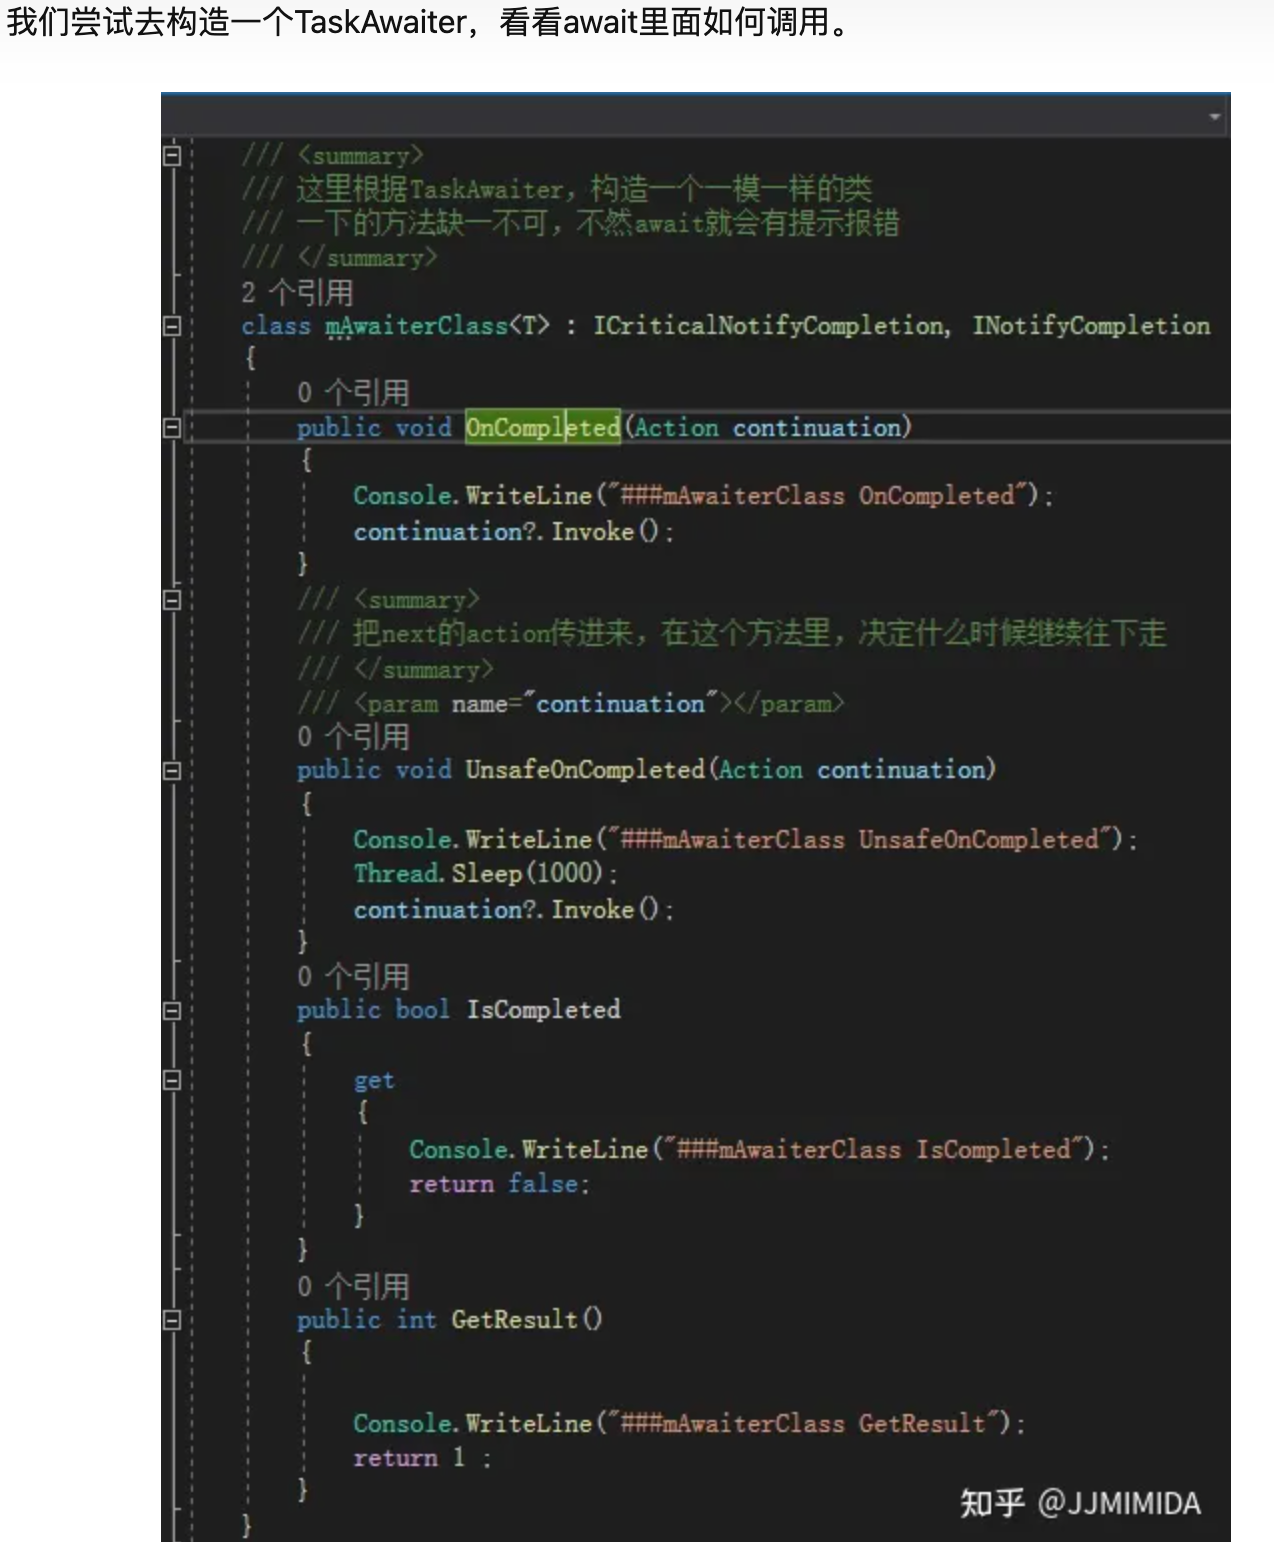
\includegraphics[width=.9\linewidth]{./pic/et3_20230609_105627.png}
\begin{itemize}
\item 它的测试用例是这么写的:注意它传入的参数类型是 int. 后面的编译码里,和它的讲解里会用到提到。
\end{itemize}

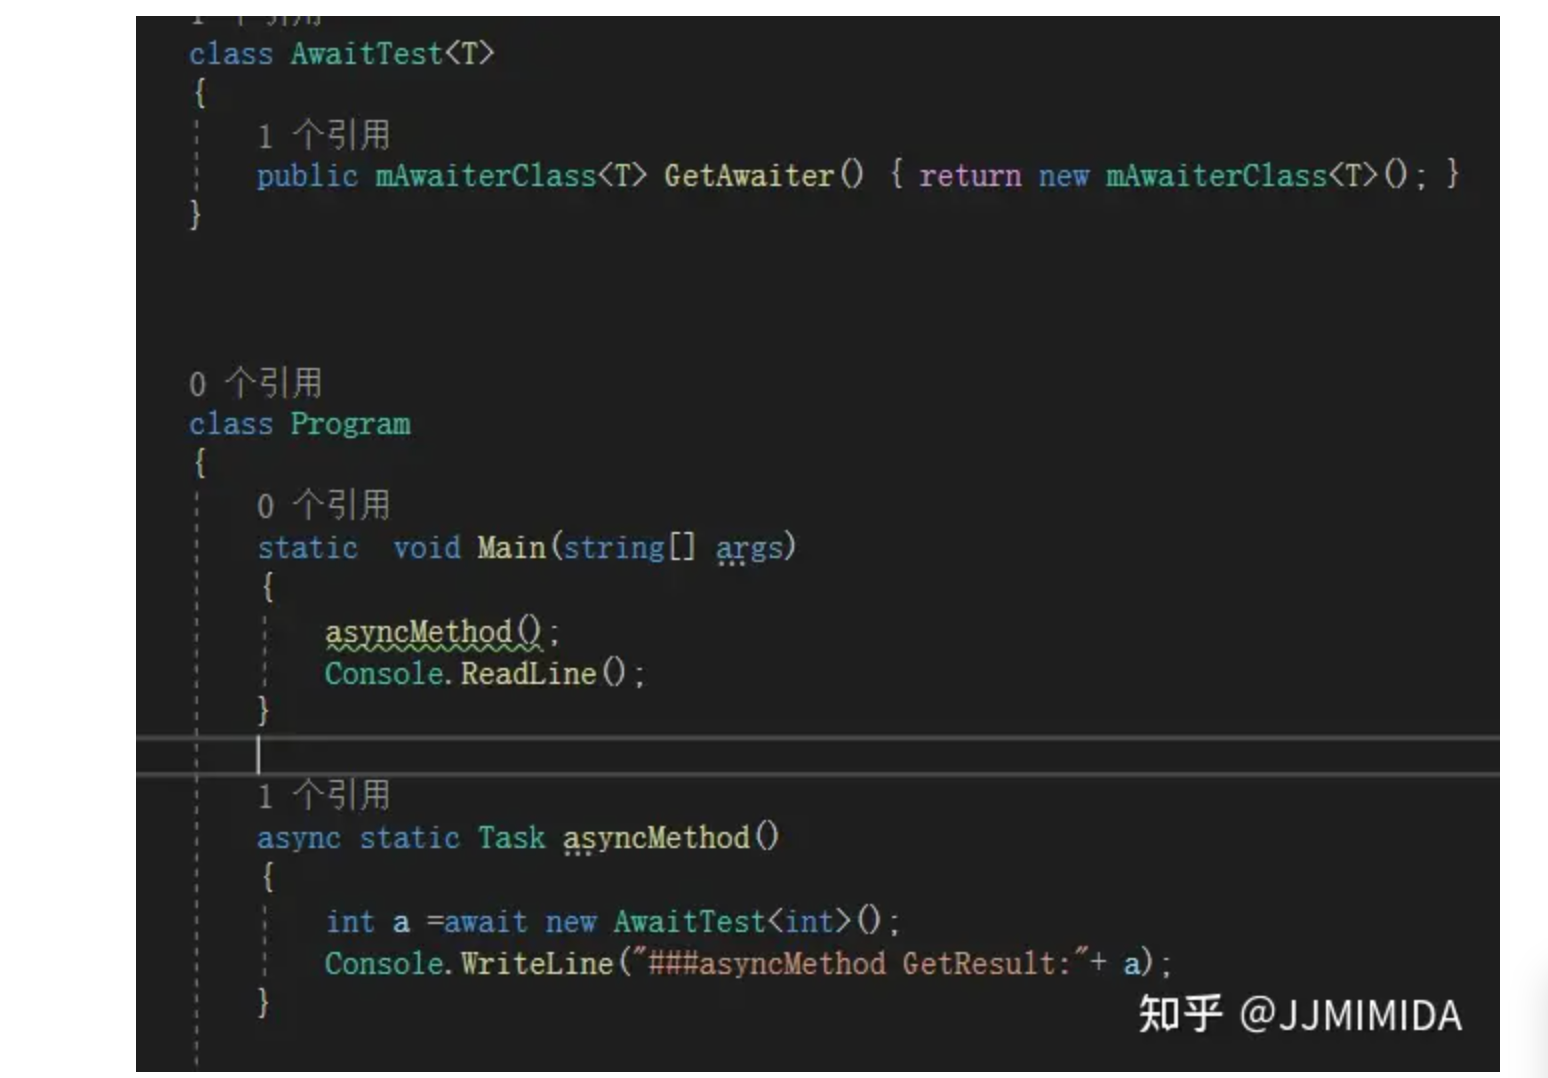
\includegraphics[width=.9\linewidth]{./pic/et3_20230609_105927.png}
\begin{itemize}
\item 看它编译出来的码(那堆编译出来的状态机的码),就是看不懂
\end{itemize}

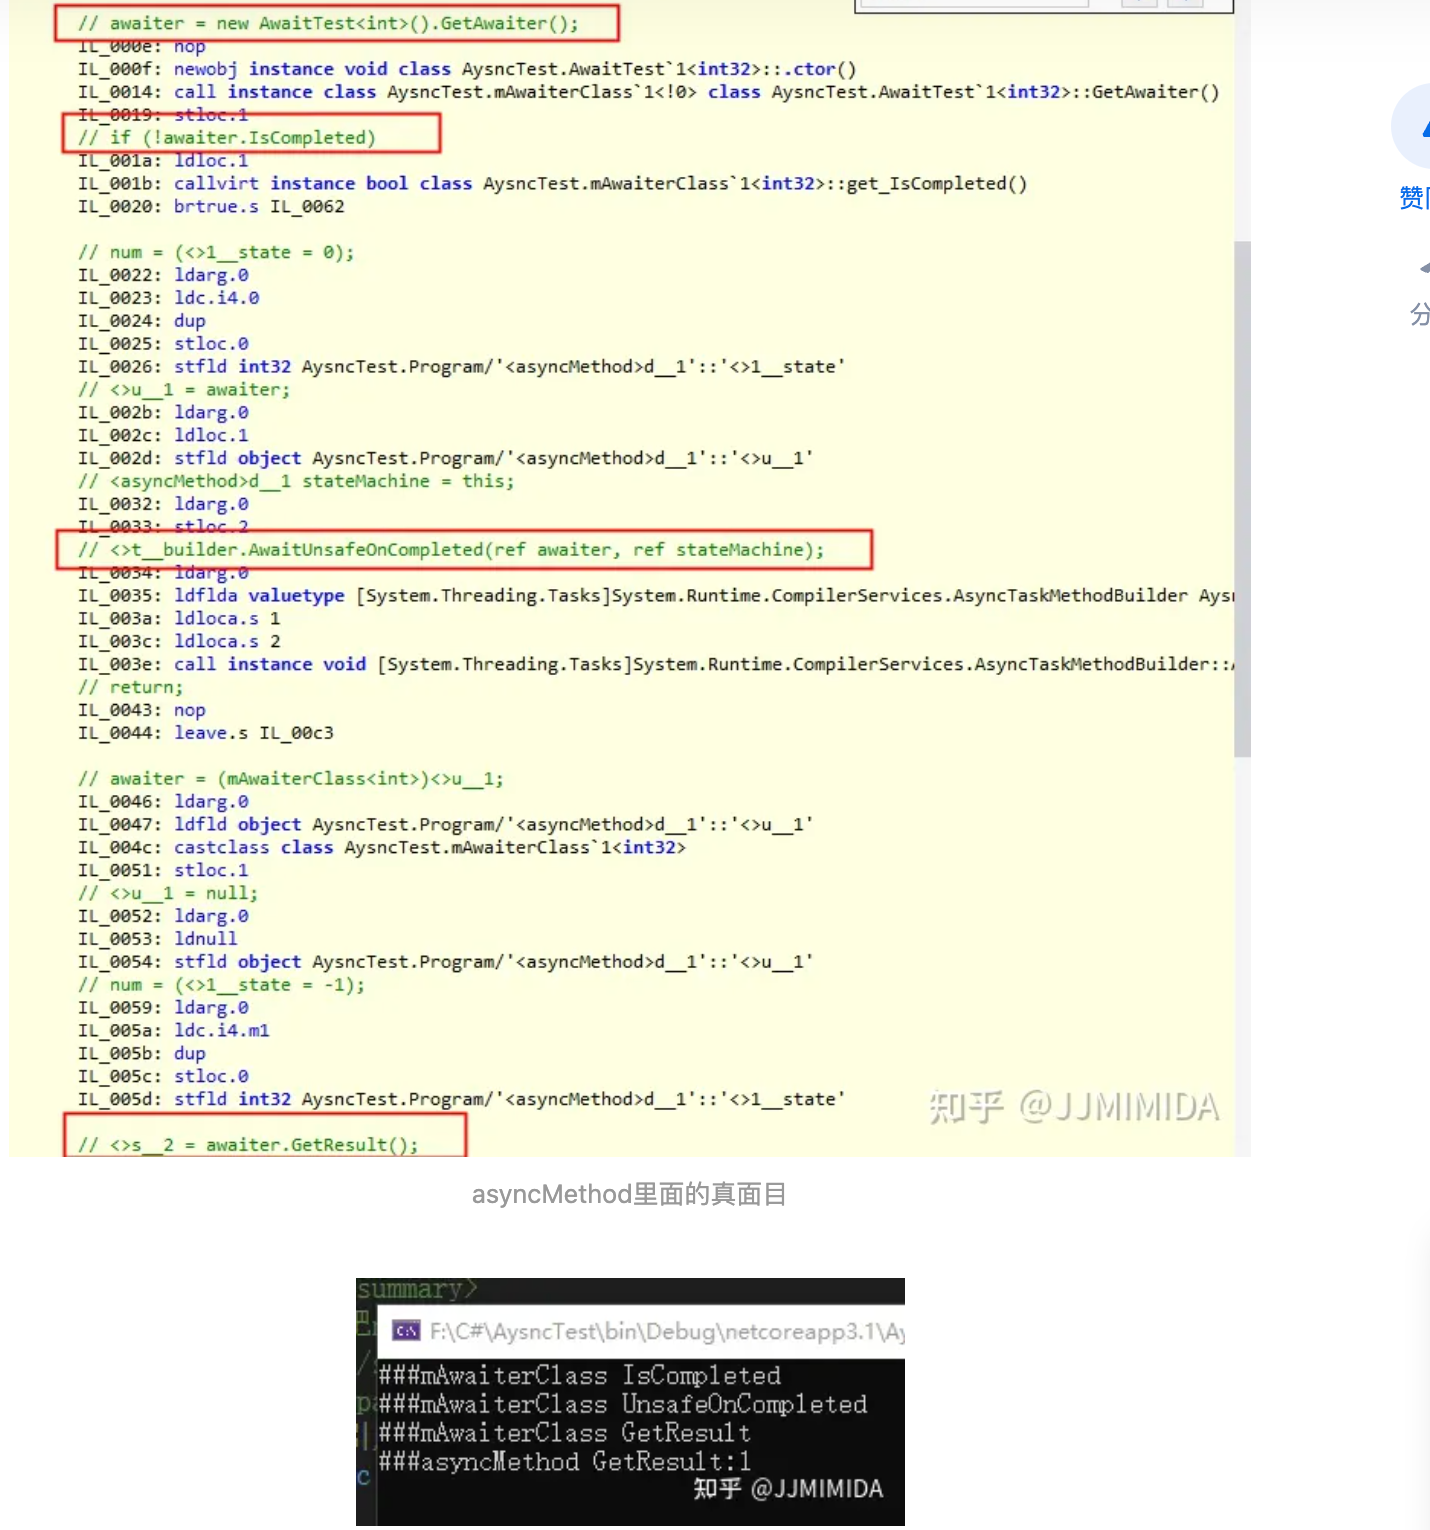
\includegraphics[width=.9\linewidth]{./pic/et3_20230609_112727.png}
\begin{itemize}
\item 结果分析: \textbf{【异步方法状态机,背后的执行顺序与逻辑:】}
\begin{itemize}
\item 先检查IsCompleted标志位,如果已经完成,则调用GetResult作为await的返回值返回。
\item 如果未完成,经过AsyncTaskMethodBuilder的AwaitUnsafeOnCompleted方法之后,最后进入UnsafeOnCompleted(nextAction),并且把完成后的下一步回调传进来。
\item 当我们获得nextAction之后,说明该调用由我们自己来控制,这里我在等待1s之后,执行nextAction(),下一步GetResult返回。
\end{itemize}
\item \textbf{【Async 关键字方法的编译原理:】}
\end{itemize}

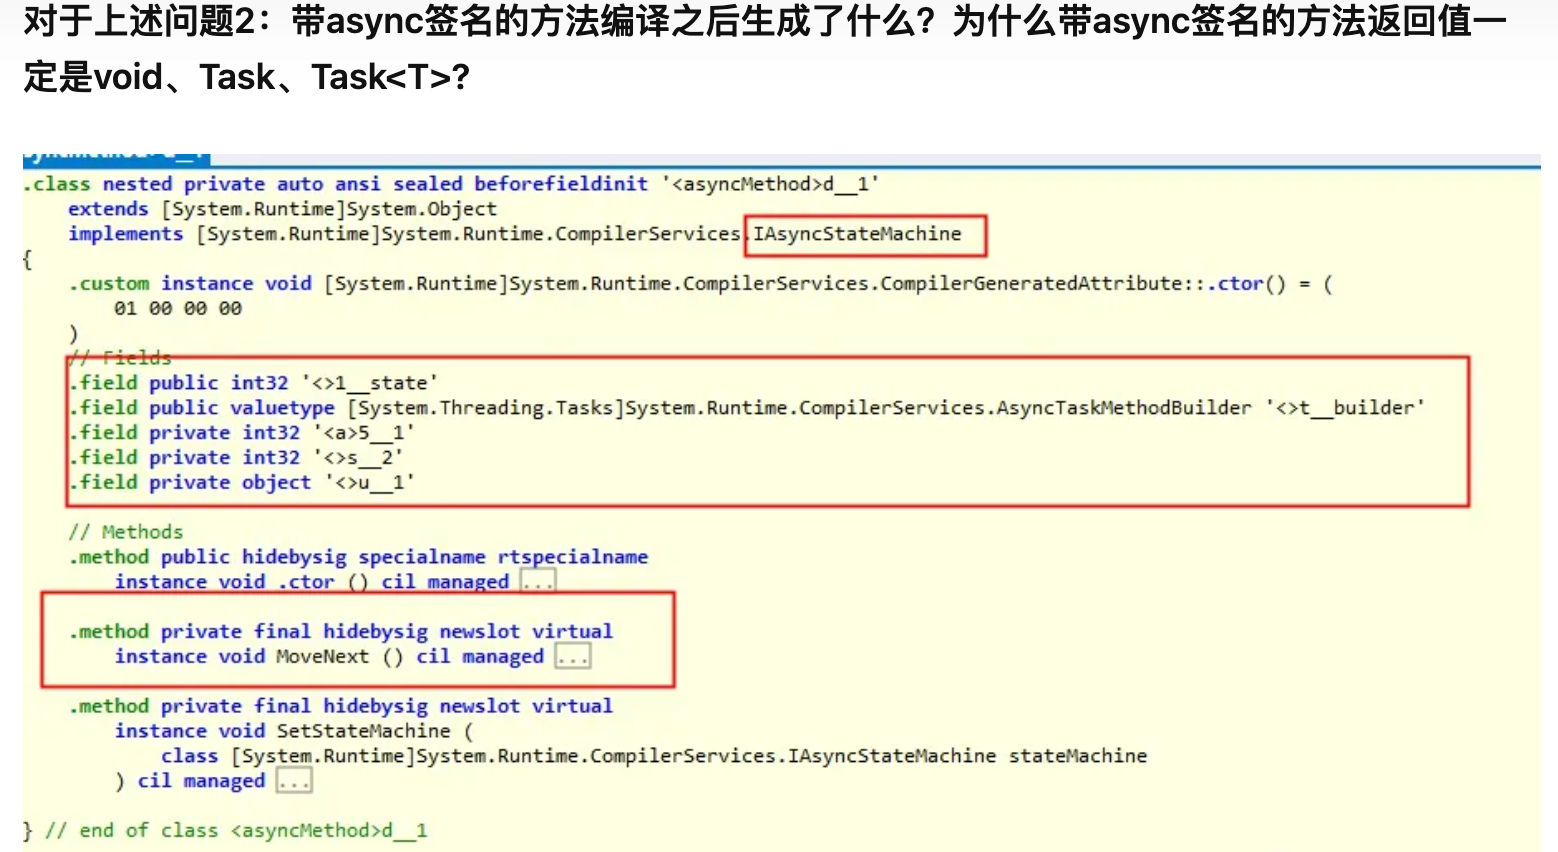
\includegraphics[width=.9\linewidth]{./pic/et3_20230609_110634.png}
\begin{itemize}
\item 这个 async 关键字所标记的异步方法,主要两个点儿: 
\begin{itemize}
\item 编译器,把这个异步方法,编译成了一个类 class <asyncMethod>d\_\_1;
\item 这个类 class, 它实现了 IAsyncStateMachine 接口,( \textbf{实现了这个接口,返回的是什么类型呢?} 这个要想明白?)
\item 这个类 class, 的内部,有几个成员变量 .field-sss.
\item 这个类 class, 的内部,有个特别重要的状态机执行函数 MoveNext() 来指挥指导,异步函数内不同节点如 await 节点等的执行逻辑。
\item 上面的逻辑,其实是就是扫描异步方法内,不同的 await 调用,每到一个这个关键字申明的异步调用,就是切换一个状态(背后有可能是线程的切换, 不一定每个分支都用不同的线程,但线程的切换可能是,必要的时候需要切换的?)分段执行。
\end{itemize}
\item 网络上的分析者还给出了下机的截图:不是狠懂,这个截图是什么意思?因为不懂,要把编译码的方法名带上,方便以后再读和理解。
\end{itemize}

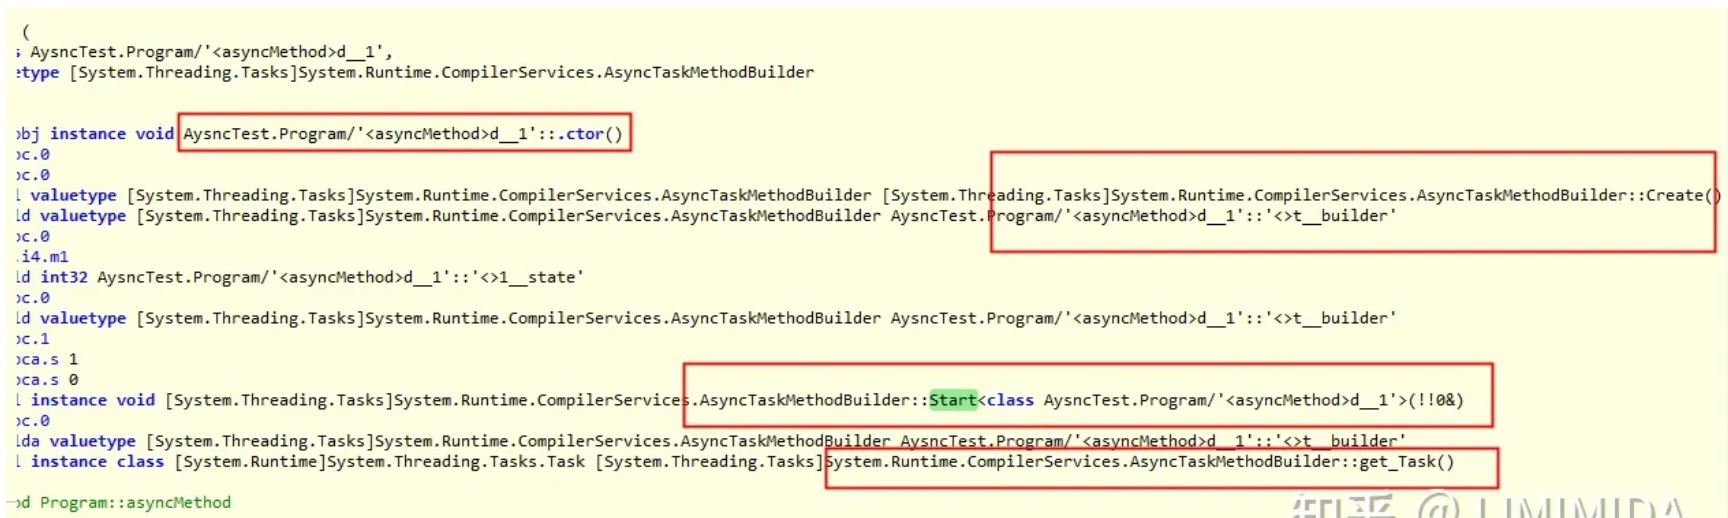
\includegraphics[width=.9\linewidth]{./pic/et3_20230609_112757.png}
\begin{itemize}
\item 上面的异步方法,所生成的异步状态机类 class 里,有几个主要的方法:
\begin{itemize}
\item 构造器方法 ctor():
\item Create() 方法:
\item Start() 方法:
\item get\_Task() 方法:
\end{itemize}
\item 可是上面的几个方法是谁,哪个接口定义的呢?
\item 网络上的分析者,对上面两个截图的分析如下: \textbf{【它讲解的这部分,我可能还是得自己编译一下,去具体看一下。】因为它的截图不完整,看不懂}
\begin{itemize}
\item 签名为async Task asyncMethod()的方法里,先创建一个继承自IAsyncStateMachine的asyncMethod类
\item 创建一个AsyncTaskMethodBuilder,然后赋值给Machine. (不知道,它这句,说的是哪里?第一个图的最后 SetStateMachine()?)
\item 初始化Machine的state = -1. (两个截图里看不见,找不到)
\item 调用AsyncTaskMethodBuilder.Start方法,start里面会进入Machine的moveNext()方法,详见问题1。
\item AsyncTaskMethodBuilder.get\_Task() 作为该方法的返回值返回。
\end{itemize}
\item 多线程问题: Task一定是多线程吗?
\begin{itemize}
\item 不一定,在上述例子中,我们定义的 async static Task<int> aa(),里面就是在同一个线程执行的。只有调用Task.Start 或者Task.Run 里面自动启用多线程的时候,才是多线程。
\end{itemize}
\end{itemize}
% Emacs 28.2 (Org mode 8.2.7c)
\end{document}